\documentclass[12pt,a4paper]{article}

\usepackage[margin=1in]{geometry}
\usepackage{setspace}
\usepackage{amsmath,amssymb,graphicx,enumerate,mathrsfs}
\usepackage{hyperref}
\usepackage{lipsum}
\usepackage{tikz}
\usetikzlibrary{arrows, positioning}

\title{\textbf{Self Referential Field Theory:\\
Explorations in Recursive Attention}}
\author{%
  Thomas Gonzalez \\
  \small \texttt{twgonzalez@deeper-truth.org}
}
\date{\today}

\begin{document}

\maketitle

\vfill
\noindent\hrulefill
\medskip

\noindent 
This work is licensed under the MIT License. You may use, copy, modify, and distribute this work provided that you include the original copyright and license notice.  For more details, see the full license text below or visit: \texttt{https://opensource.org/licenses/MIT}.
\medskip \\
\rightline{\textbf{\textcopyright~2025 Thomas Gonzalez}}

\newpage

\begin{abstract}
This paper introduces a speculative Self Referential Field Theory (SRFT) that offers both an ontological stance and a generative mechanism for understanding consciousness and reality. At the ontological level, the SRFT posits a \textbf{primordial, unbounded Awareness Field}---a field of pure potentiality analogous to a superposition, encompassing all possibilities of experience, form, and structure---existing prior to and independent of spacetime. Building on insights from Eastern non-dual philosophies and Western process thought, the theory explains \emph{how} this single underlying Awareness can differentiate into myriad forms—physical structures, mental states, and social phenomena. This is achieved through the mechanism of \textbf{recursive Attention}, an intrinsic, self-referential force that ``folds'' the Awareness Field upon itself, iteratively actualizing latent potentials. This dynamic is mathematically captured by the Seed Equation: \(\mathscr{A}^\infty = \mathcal{H}(\mathscr{A}^\infty) \sim \mathscr{A}^\infty\), where \(\mathscr{A}^\infty\) represents the Awareness Field, \(\mathcal{H}\) the harmonic operator encoding its resonant modes, and \(\sim\) the convolution operator representing self-interaction. The folding process, much like a wave crashing upon itself, stabilizes into coherent wave-like attractors---the phenomena that constitute our experienced reality---and gives rise to the flow of emergent time.

By drawing an analogy with how \( \sin \) and \( \cos \) arise intrinsically from circular geometry, we suggest that wave-like phenomena and recursive dynamics may likewise be \emph{intrinsic} to this unbounded Awareness Field. Rather than relying solely on a “water-ripple” metaphor, we emphasize that waves can exhibit both stable and disruptive phases, effectively “crashing” and re-injecting energy (or probability) back into the system, leading to transient attractors that may then be reabsorbed. \textbf{The SRFT's novel contribution lies in its conceptualization of recursive Attention as a fundamental, iterative process driving the emergence of all phenomena.}

We situate the SRFT in relation to Ken Wilber’s Integral Theory, Alfred North Whitehead’s process philosophy, and various panpsychist or neutral monist perspectives, noting how SRFT’s explicit focus on \emph{recursion} and \emph{self-perturbation} extends beyond these earlier approaches.

While the discussion remains primarily conceptual, we suggest directions in which the SRFT might inform scientific and philosophical inquiry—ranging from the “hard problem” of consciousness to large-scale social dynamics. We also highlight potential applications in artificial intelligence, particularly in understanding how consciousness might emerge in artificial systems. Through examples in mental state regulation, collective behaviors, and scale-invariant fractal features evident in the physical universe, we illustrate how recursive Attention could unify a broad spectrum of phenomena. By reframing mind and matter as \textbf{emergent attractors} within an \textbf{unbounded Awareness Field}, the SRFT invites further research in both theoretical and empirical domains, with the hope of bridging enduring gaps between spirituality, philosophy, and science.
\end{abstract}

\section*{Author's Note}

The nature of consciousness and its relationship to the physical world remains one of the most profound and enduring mysteries in both science and philosophy. This pre-print introduces the \emph{Self Referential Field Theory} (SRFT), a speculative framework positing an “unbounded Awareness Field” as the foundation of all existence. My path to this theory began decades ago, prompted by early studies in philosophy, Buddhism, and computer science, and was further shaped by my experiences in neural networks, software engineering, and meditation practice.

Though I hold an undergraduate degree in visual arts and have pursued studies in computer science at UCSD, my insights also stem from working as an entrepreneur, artist, and executive coach for over twenty-five years. These varied roles fueled my interest in how \emph{attention} and \emph{awareness} influence both individual cognition and broader social systems. While I have no formal training in philosophy, neuroscience, advanced mathematics, or theoretical physics, I offer here an “architectural sketch” rather than a finalized theory—one that benefits from my interdisciplinary background and ongoing dialogue with contemplative and scientific perspectives.

At the heart of the SRFT is “recursive Attention,” a self-referential process through which the Awareness Field differentiates into myriad forms. Although this paper remains speculative, I hope it sheds fresh light on longstanding questions about the mind–matter relationship and the evolution of consciousness. I invite collaboration and critique from scientists, philosophers, mathematicians, and practitioners from every field to help refine these ideas. My aspiration is that such collective efforts will yield a deeper, integrated understanding of ourselves, the universe, and our shared interconnections.

Lastly, I acknowledge that much of the reading, referencing, and preliminary drafting for this paper was accelerated by AI tools (including large language models), which enabled me to integrate diverse sources and refine arguments more quickly.

\newpage
\tableofcontents
\newpage

\section{Introduction}
\label{sec:intro}

\subsection{Motivation: Why a New ``Self Referential Field Theory''?}
Questions surrounding the nature and origin of consciousness and our physical reality continue to challenge both philosophy and science. Despite remarkable advances in neuroscience and cognitive science, there is no widely accepted account of how subjective experience (the ``felt'' dimension of mind) arises from, or coexists with, the physical domain. Many existing models capture important features of consciousness—ranging from predictive processing to complex information integration—yet a unified account that explains the multiplicity of phenomena \textbf{across all scales and domains}—\textbf{from subjective perceptions and thoughts to social dynamics, biological systems, and the fundamental structure of the physical universe}—and how they might share a more fundamental ground remains elusive.

It is within this context that we propose a speculative \emph{Self Referential Field Theory (SRFT)}, which draws on non-dual philosophical traditions as well as Western process thought. We aim to offer a conceptual lens that treats ``Awareness'' as \textbf{a universal field of potentiality}, out of which distinct forms emerge through a self-referential intrinsic drive we call ``recursive Attention.'' \textbf{The SRFT seeks to move beyond theories that focus solely on the mind-body problem and instead offers a framework for understanding the emergence of all phenomena from a unified field of awareness.} This is not merely an exercise in abstract metaphysics, but rather a necessary step towards developing a truly comprehensive and integrated understanding of reality that includes not only physical systems, but also the richness and complexity of subjective experience and the dynamics of biological, social, and cultural systems.  To ground this theory in a rigorous mathematical framework, we have developed a novel partial differential equation (PDE) that models the dynamics of the Awareness Field. \textbf{This PDE, presented in its ``Seed'' form as \(\mathscr{A}^\infty = \mathcal{H}(\mathscr{A}^\infty) \sim \mathscr{A}^\infty\), incorporates fractional calculus, dynamic dimensionality, and a convolution operator to capture the self-referential, recursive nature of Attention.  Preliminary mathematical analysis and proof sketches for the well-posedness of this equation are detailed in this COMPANION PAPER.} While this work is ongoing, these initial results lend credence to the SRFT's core premise. In contrast to purely materialist or idealist accounts, the SRFT aspires to reconcile the unity of an underlying \textbf{Awareness Field} with the multiplicity of concrete phenomena.

\vspace{1em}
\noindent\textbf{Guided Thought Experiments (Companion Paper).}
To provide a more \emph{intuitive} grasp of these ideas, we have published a set of \emph{Guided Thought Experiments} separately 
(\emph{``Self-Guided Thought Experiments: From a Simple Pond to a Vast `Awareness Ocean' ''}). These exercises walk readers through a water-ripple metaphor step by step, illustrating how recursive wave interactions in an “awareness ocean” might give rise to stable attractors (e.g., physical forms, mental states, and social patterns). While this paper focuses on the 
SRFT’s theoretical foundations, readers seeking a hands-on, imaginative introduction to wave-based emergence and the role of attention may find the Guided Thought Experiments a helpful companion.


\subsection{Existing Debates on Consciousness: The Hard Problem, Free Will, and the Combination Problem}

In modern consciousness studies, the so-called ``hard problem'' \cite{chalmers1995} points to the difficulty of explaining why and how we have subjective phenomenal experiences at all. While certain frameworks (e.g., Global Workspace Theory \cite{baars1988}; Integrated Information Theory \cite{tononi2008}; Predictive Processing \cite{friston2010}) successfully elucidate neural correlates or cognitive architectures, they often leave open the deeper ontological question of 
\emph{why} these correlates yield phenomenal experience rather than a purely unconscious information flow. Moreover, panpsychist accounts \cite{skrbinapsp} propose consciousness as ubiquitous but grapple with combining individual “micro-experiences” into a unified macro-experience (the ``combination problem''). Within this broad landscape, non-dual philosophical traditions---
including Advaita Vedanta and certain strands of Mahayana Buddhism---have long emphasized the primacy of a singular awareness prior to any subject--object distinction, yet they often remain at a conceptual distance from contemporary scientific discourse.

\paragraph{}
In addition to the \emph{hard problem} and the \emph{combination problem}, questions of \textbf{agency and free will} remain pivotal. Many theories describe \emph{how} cognition occurs but say little about \emph{why} we experience ourselves as causal agents—or whether that sense of agency is fully compatible with physicalist or panpsychist models. We revisit these challenges 
and propose a unifying perspective on \textbf{agency and free will} in Section~\ref{sec:agency-freewill}.


\subsection{Novel Contribution: Ontological Basis \& Generative Mechanism}

The central proposition of the SRFT is that \emph{recursive Attention} acts as a generative mechanism. While the notion of an underlying \textbf{Awareness Field} echoes elements of non-dual and process philosophies, we develop a specific claim: that ``Attention'' is more than a localized cognitive act (as typically discussed in psychology or neuroscience). Rather, it is an intrinsic, self-referential process that “selects” or amplifies certain latent potentials, thereby stabilizing them into coherent wave-like patterns or “attractors.” \textbf{In other words, our approach extends non-dual metaphysics by providing both (a) an \emph{ontological} foundation (the unbounded Awareness Field) and (b) a \emph{mechanistic} explanation (recursive Attention) for how diverse phenomena arise.} By analogy with other wave phenomena (e.g., how \(\sin\) and \(\cos\) emerge intrinsically in circular geometry), we suggest that such recursive dynamics may be \emph{integral} to the unbounded Awareness Field itself. This perspective not only accounts for the apparent multiplicity of manifest phenomena but also suggests a way to integrate subjective consciousness, physical laws, and even social structures into a single emergent framework.

\subsection{Roadmap of the Paper}

Having introduced the Self Referential Field Theory (SRFT) in the preceding section and highlighted key challenges in consciousness studies (e.g., the “hard problem,” free will, and the combination problem), we now turn to a more detailed examination of existing philosophical and scientific approaches. We have also laid out our \emph{novel contribution}, which unifies an \emph{unbounded Awareness Field} (ontology) with \emph{recursive Attention} (mechanism). 

The remainder of this paper proceeds as follows. In \textbf{Section~\ref{sec:lit-review}}, we situate our proposal within broader philosophical and scientific debates, including dualism, physicalism, panpsychism, process philosophy, and integral theory. This background clarifies where the SRFT 
diverges from or extends existing frameworks.

\textbf{Section~\ref{sec:core-foundations}} then presents the core theoretical underpinnings of the SRFT, introducing key terms (\emph{Awareness}, \emph{Attention}, \emph{Stable Attractors}) 
and spelling out our central ontological commitments. Building on these foundations, we explore how phenomena—ranging from subatomic to societal—could arise within a timeless Awareness Field.

In \textbf{Section~\ref{sec:convolution-core}}, we shift to the mechanism of SRFT and detail the “convolution-like” dynamic through which the Awareness Field continually folds back on itself to generate emergent patterns and the sense of time. \textbf{Section~\ref{sec:harmonics-core}} complements this by examining the wave-like or harmonic processes (\(\mathcal{H}\)) that interact with recursive Attention, forming stable modes or attractors.

Shifting focus to \emph{emergent phenomena}, \textbf{Section~\ref{sec:emergent-features}} shows how new forms take shape via iterative selection and why certain patterns—such as social memes, neural oscillations, or physical structures—endure. We then address foundational debates about consciousness and volition in \textbf{Section~\ref{sec:key-debates}}, illustrating how the SRFT might shed light on the hard problem of consciousness and the nature of free will or agency.

With these elements in place, \textbf{Section~\ref{sec:SRFT-detailed}} revisits the theory with greater rigor, re-examining the water-ripple metaphor, proposing potential empirical research, and drawing comparisons with other prominent theories of mind and reality. Anticipating key criticisms, \textbf{Section~\ref{sec:counterarguments}} surveys typical objections—such as circular reasoning and the sweeping scope of the theory—and offers preliminary replies.

\textbf{Section~\ref{sec:applications-extensions}} explores how the SRFT’s central ideas might apply in neuroscience, complex social systems, transpersonal psychology, and the study of scale-invariant fractal processes. Afterward, \textbf{Section~\ref{sec:future-work}} outlines pathways for further theoretical refinement, empirical exploration, and cross-disciplinary collaboration, including advanced PDE modeling and astrophysical simulations of fractal patterns.

Finally, \textbf{Section~\ref{sec:conclusion}} summarizes our  principal contributions, emphasizing the potential of an “awareness-first” approach to unify a wide range of phenomena and research fields. In doing so, we reiterate that while the SRFT remains speculative, it provides a conceptual framework that invites deeper inquiry into the nature of consciousness and reality.

\medskip
\noindent
\textbf{Note on Broader Speculations.} 
This paper also speculates on potential implications in astrophysics (e.g., cosmic dust formation, black-hole information), fractal PDE modeling, and advanced AI or LLM-driven systems. These connections remain highly exploratory but illustrate the wide scope of \emph{recursive Attention} as a universal principle. We offer them not as confirmed predictions but as invitations for interdisciplinary collaboration, demonstrating how the SRFT’s core concepts might intersect with frontier questions in physics, mathematics, and compSRFTtional science.
\medskip

\subsection{Motivation and Context}
\label{sec:motivation-context}

The study of consciousness poses a unique challenge within both scientific and philosophical domains. On one hand, researchers in neuroscience and cognitive science have made great strides in mapping neural correlates of consciousness, elucidating functional architectures such as the Global Workspace \cite{baars1988} or the free-energy principle \cite{friston2010}. On the other hand, these empirical advances do not fully account for the \emph{qualitative} aspect of subjective experience, a gap often highlighted by the so-called ``hard problem'' of consciousness \cite{chalmers1995}. Efforts to resolve this explanatory gap have led to various theoretical standpoints, including physicalism, property dualism, and panpsychism, yet consensus remains elusive.

Beyond the mainstream discourse, a range of non-dual philosophical traditions (e.g., Advaita Vedanta, certain forms of Mahayana Buddhism) and process-oriented frameworks (e.g., Whitehead’s Process and Reality) propose that the multiplicity of phenomena emerges from a deeper, unbounded Awareness field underlying reality. According to these views, the perceived boundaries between subject and object, or between mind and matter, may be conceptual overlays on an underlying oneness. While such approaches are often deemed metaphysical or speculative, they offer a valuable lens for reevaluating how consciousness, as a universal field or principle, could give rise to the world we perceive.

In this paper, we draw upon these insights to formulate a \emph{Self Referential Field Theory (SRFT)}. Our motivation stems from a desire to integrate the strengths of contemporary scientific theories---which excel at describing \emph{how} consciousness functions and correlates with neural structures---with the holistic perspective of non-dual and process philosophies, which emphasize \emph{why} all manifest forms might arise from a singular, \textbf{unbounded Awareness}. By introducing the concept of \emph{recursive Attention} as an intrinsic generative mechanism, we aim to bridge these domains and explore a potential path toward reconciling the diversity of phenomena (physical, psychological, and social) with an underlying continuity.


\section{Background and Literature Review}
\label{sec:lit-review}

This section places our \emph{Self Referential Field Theory (SRFT)} in relation to historical and contemporary debates in philosophy and consciousness studies. We begin by surveying the principal philosophical stances on mind and matter, then review leading scientific theories of consciousness, and conclude with an examination of process philosophy, integral theory, and other integrative frameworks that resonate with our approach.

\subsection{Philosophical Context: Dualism, Monism, and Beyond}
\label{subsec:philosophical-context}

The mind--body problem has long been a central puzzle in Western philosophy \cite{descartes1641}, traditionally framed as a tension between mental phenomena and the physical world. 
\begin{itemize}
    \item \textbf{Substance Dualism:} Tracing back to Descartes, substance dualism posits that mind and matter belong to fundamentally different substances \cite{descartes1641}. While it acknowledges the reality of subjective experience, it struggles to explain the causal interaction between the two domains without invoking ad hoc mechanisms.
    \item \textbf{Physicalism (Materialism):} Physicalist views hold that all phenomena, including consciousness, can ultimately be reduced to or supervene on physical states. Prominent versions include eliminative materialism and reductive functionalism \cite{churchland1989}. These have had significant traction in neuroscience but often leave the ``hard problem'' of subjective experience unresolved \cite{chalmers1995}.
    \item \textbf{Panpsychism and Neutral Monism:} Partly in response to physicalism's explanatory gaps, panpsychism proposes that a form of proto-consciousness is present in all matter \cite{skrbinapsp}. Meanwhile, neutral monism (endorsed historically by James, Mach, and Russell) suggests a single, more fundamental ``neutral'' stuff that underpins both mind and matter \cite{mach1886analysis, russell1921analysis}. Despite providing a unifying metaphysical layer, panpsychist and neutral-monist accounts can face the ``combination problem,'' namely how individual micro-conscious elements combine into a unified macro-consciousness.
    \item \textbf{Non-Dual Traditions:} Eastern philosophies like Advaita Vedanta or certain Mahayana Buddhist schools propose that all apparent distinctions emerge from (and dissolve back into) a singular, non-dual reality \cite{ramacandra1923upanishads, garfield2002emptiness}. While often couched in spiritual rather than scientific discourse, these frameworks place emphasis on direct experiential insight and the illusory nature of dualities (subject--object, mind--body).

    \item \textbf{Hoffman’s Conscious Realism:}
    Donald D.~Hoffman proposes that our sensory perceptions function like an evolutionary ``user interface'' rather than a truthful depiction of an objective world, suggesting consciousness or conscious agents underlie reality \cite{hoffman2015,hoffman2019case}. While Hoffman's model has not been widely adopted
    in mainstream neuroscience, it resonates with ``awareness-first'' perspectives by treating matter as secondary to mind. However, like many non-physicalist frameworks, it faces challenges in fully specifying how subjective experiences take shape at each scale of analysis.
\end{itemize}

Against this philosophical backdrop, our own approach locates itself closer to a non-dual or neutral monist position. However, the \emph{SRFT} introduces a distinctive emphasis on \emph{recursive Attention}---suggesting a self-referential intrinsic drive that shapes emergent phenomena from a \textbf{fundamental, unbounded Awareness Field}. This perspective not only recalls classic debates about an all-encompassing “substrate” in traditional metaphysics but also reconfigures them around the question of how unity differentiates into multiplicity.

\subsection{Contemporary Theories of Consciousness}
\label{subsec:consciousness-theories}

Shifting to modern scientific discourse, numerous theories attempt to explain \emph{how} consciousness arises or is maintained in neural systems:

\begin{itemize}
    \item \textbf{Global Workspace Theory (GWT):} 
    Proposed by Baars \cite{baars1988} and further developed by others (e.g., Dehaene), GWT posits that consciousness emerges when information becomes globally available in a ``workspace'' that integrates multiple specialized processes. While GWT robustly accounts for the functional role of attention, it stops short of explaining \emph{why} integrated information feels like something from the inside.

    \item \textbf{Integrated Information Theory (IIT):} 
    Tononi’s \cite{tononi2008} IIT defines consciousness in terms of the quantity and quality of integrated information ($\Phi$). By attempting to measure ``how unified'' and ``how differentiated'' a system’s internal states are, IIT offers a potential bridge between phenomenology and physical substrate. Critics, however, point out that IIT’s axioms risk being too abstract or difficult to validate empirically, and that it does not fully resolve the ontological status of experience.

    \item \textbf{Predictive Processing and Free-Energy Principle:} 
    Friston’s free-energy principle \cite{friston2010} and related ``predictive processing'' accounts see the brain as a prediction-making organ that minimizes surprise by updating its internal models of the world. Although these frameworks illuminate functional aspects of perception and cognition, the leap from Bayesian inference to first-person consciousness is often underspecified.

    \item \textbf{Higher-Order Theories:} 
    Other approaches, such as Higher-Order Thought Theory (HOT) or Higher-Order Perception Theory (HOP), suggest that a mental state becomes conscious when one has a higher-order representation of it \cite{rosenthal2005}. While this captures introspective awareness, debates continue over whether higher-order representations are necessary or sufficient for phenomenal experience.
\end{itemize}

Each of these theories proposes important mechanisms—global broadcasting, information integration, predictive coding, higher-order representation—that contribute to our scientific understanding of consciousness. Nevertheless, many still confront the \emph{explanatory gap} regarding the intrinsic \emph{feel} of experience. In the SRFT, by contrast, we explore how \emph{Awareness} might itself be primary, with emergent forms and laws arising through an internal process of recursive self-selection. From this vantage, standard theories of consciousness might be seen as describing particular \emph{facets} or \emph{local instantiations} of a more \textbf{awareness-based} dynamic.

\subsection{Process Philosophy, Integral Theory, and Related Frameworks}
\label{subsec:process-integral}

Philosophical movements that foreground \emph{process} over static substance can serve as bridges between traditional metaphysics and contemporary science:

\begin{itemize}
    \item \textbf{Whitehead’s Process Philosophy:} 
    In \emph{Process and Reality}, Alfred North Whitehead \cite{whitehead1929process} posited that reality is fundamentally composed of events or ``actual occasions,'' each incorporating and prehending the others. Whitehead’s radical emphasis on becoming rather than being parallels the SRFT’s notion of emergent phenomena, suggesting that the world is an ongoing interplay of processes rather than a collection of inert objects.

    \item \textbf{Ken Wilber’s Integral Theory:}
    Wilber’s work \cite{wilber1995sex, wilber2007integral, wilber2000brief} integrates subjective, intersubjective, objective, and interobjective perspectives into a comprehensive framework. One of Wilber’s central principles is “transcend and include,” in which each developmental stage both surpasses and incorporates earlier stages. While Wilber’s emphasis on multiple quadrants acknowledges the complexity of human experience, the SRFT adds a more explicit claim about the underlying \emph{mechanism} (recursive Attention) that explains \emph{how} these diverse layers might cohere into a single reality.
    
    In this sense, Wilber’s “transcend and include” aligns with the SRFT’s notion of self-referential “folding in,” wherein new emergent forms build upon and integrate prior states within the unbounded Awareness Field. Moreover, Wilber sometimes refers to an evolutionary \emph{drive} or “Eros” that propels each level of development into a fuller manifestation. The SRFT parallels this by proposing that \emph{Attention} itself is an \emph{intrinsic impetus}—both establishing the “is-ness” of each moment and \emph{catalyzing} further differentiation. While Wilber’s “Eros” is often described in more spiritual or teleological terms, the SRFT treats recursive Attention as a \emph{mechanistic} (yet deeply ontological) driver that continually ‘folds’ the Awareness Field into new emergent forms.
    
    \item \textbf{Transpersonal and Non-Dual Frameworks:} 
    Various transpersonal psychologists and non-dual philosophers (e.g., Sri Aurobindo, Ramana Maharshi, certain Dzogchen traditions) have argued that consciousness itself is the ontological ground of existence \cite{ramacandra1923upanishads, garfield2002emptiness}. While traditionally positioned on the edges of mainstream academic discourse, their emphasis on direct experiential insight and the dissolution of subject--object dualities resonates strongly with the SRFT’s central thesis that \textbf{Awareness} is fundamental.
\end{itemize}

By weaving together insights from process philosophy and integral approaches, we aim to go one step further in positing a \textit{recursive force}---\emph{Attention}---which could clarify the \emph{mechanism} by which an undifferentiated Awareness self-manifests as myriad forms. Process thought supports the idea that reality is dynamic and relational, and integral theory highlights the multidimensionality of human understanding. The SRFT attempts to situate these intuitions in a single conceptual framework, recognizing that the multiplicity of phenomena across physical, mental, and social domains might indeed be traced back to the same underlying principle of self-referential \emph{convolution} (sometimes described as “folding in” or “perturbation”).

\paragraph{Summary of Connections.}
In sum, the SRFT shares philosophical ground with panpsychism, neutral monism, process metaphysics, and integral thinking, while attempting to address the enduring challenge of describing \emph{how} unity gives rise to apparently distinct, emergent patterns. Contemporary theories of consciousness provide a partial map of \emph{functional} mechanisms, but they rarely tackle the underlying ontology of experience. Our next step is to articulate the core definitions and ontological commitments of the SRFT itself, before exploring its potential implications.

\medskip
 
As we shall see, the SRFT introduces a \emph{Seed Equation} (Section~\ref{subsec:seed-equation}) to symbolically capture how wave-like (harmonic) interactions within an unbounded Awareness Field might “convolve” or fold in on themselves through the intrinsic drive of Attention. While we do not reduce consciousness to mere wave equations, this language underscores the possibility of emergent patterns—akin to how $\sin$ and $\cos$ appear in circular geometries—that may be further explored using tools from complexity science, and even, in principle, advanced mathematics such as fractional PDEs. The next sections will develop these ideas more fully.

\section{Core Theoretical Foundations}
\label{sec:core-foundations}

In this section, we present the foundational concepts of the Self Referential Field Theory (SRFT), clarifying its key definitions, ontological commitments, and the central notion of \emph{recursive Attention}. These pillars collectively aim to explain how a \textbf{universal field of Awareness} can, through self-referential processes, give rise to emergent phenomena across mental, physical, and social domains---including the dimension we call ``time.'' In particular, we distinguish an \textbf{\emph{ontological claim}} (that an unbounded Awareness Field underlies all phenomena) from a \textbf{\emph{mechanistic principle}} (that `recursive Attention' drives the emergence of discrete forms and experiences).


\subsection{Key Definitions}
\label{subsec:key-defs}

\paragraph{Clarifying Terminology.} 
Although many theories might call this a “substrate,” we avoid that term here to prevent confusion with purely physical or material bases. Instead, we emphasize the \textbf{Awareness} Field as a metaphysical source of all latent possibilities rather than a physical layer. In this sense, it resembles the idea of \emph{potentiality} in quantum theory, where multiple states may coexist in superposition before any ‘collapse’ or selection. However, we do not literally equate the Awareness Field with quantum wavefunctions; the term ‘unbounded Awareness’ simply underscores a \emph{boundless continuum of potential} rather than a static substrate confined by physical laws. Throughout this paper, we will use “Awareness Field” and “unbounded Awareness” somewhat interchangeably to denote this same fundamental reality.


\subsection{Ontological Commitments}
\label{subsec:ontological-commitments}

\subsubsection{Awareness-Based Ontology (Neutral Monism or Non-Dual)}
The SRFT adopts a stance reminiscent of \emph{neutral monism} or \emph{non-dual} philosophy. Rather than labeling reality as purely mental or purely physical, we assert that these categories both emerge within a more fundamental \emph{Awareness Field} of potentiality. In doing so, we diverge from materialist accounts (where consciousness is a latecomer byproduct of purely physical processes) and from classical idealism (where mind precedes all physicality).


\subsubsection{Attention (in a Metaphysical Sense)}
\label{subsubsec:attention}

Whereas conventional psychology often treats attention as a localized cognitive process, in the SRFT we adopt a more \emph{metaphysical} usage. \emph{Attention} is the intrinsic, self-referential creative drive of the \textbf{Awareness Field} (or Ground Potentiality) to ``select'' or ``amplify'' latent potentials, effectively bringing them into manifestation. Rather than occurring in a pre-existing time, \emph{Attention} \emph{creates} the sense of time whenever it iterates upon itself in a self-reflexive cycle.

\subsubsection{Space and Time as Emergent}
A key ontological claim is that space and time are not pre-given frameworks but \emph{arise} through repeated “folding in” or convolution of the \textbf{unbounded} Awareness Field. Because \emph{space} and \emph{time} themselves are posited to emerge 
within (rather than prior to) this Awareness Field, one must be careful when referring to “processes” or “iterations.” From the ultimate vantage point (i.e., the unbounded Awareness Field), there are no spatial or temporal coordinates. Nevertheless, once the 
field differentiates, the dimension of time—and with it, the notion of \emph{sequences} or \emph{iterations}—arises as an aspect of emergent phenomena.

When we speak of “things happening over time,” we therefore describe phenomena from the \emph{emergent} vantage point, in which time is already a dimension. From the fundamental perspective, such processes do not occur \emph{in} a pre-existing timeline; rather, they \emph{generate} the experienced continuity that we label “time.”


\paragraph{Connectivity Across Emergent Timelines}
Even though time is an emergent feature, the unbounded nature of Awareness implies that all events, past and future, remain embedded in and connected via the underlying field. This helps explain how memory, causality, and other seemingly time-dependent phenomena might retain coherence. The \emph{recursive convolution} of the field through Attention ensures that emergent events are never fully severed from the \textbf{unbounded Awareness Field} or from each other.




\subsection{The Seed Equation as a Conceptual Bridge}
\label{subsec:seed-equation}

\noindent
\textbf{Motivation.} 
Although this paper remains primarily conceptual, a simple symbolic expression can help us visualize how the unbounded Awareness Field might “fold in” on itself to yield stable forms. We refer to this expression as the \emph{Seed Equation}:


\
\[
\mathscr{A}^\infty = \mathcal{H}(\mathscr{A}^\infty) \;\sim\; \mathscr{A}^\infty
\]



where:
\begin{itemize}
    \item \(\mathscr{A}^\infty\) denotes the unbounded ``Awareness Field,'' an infinite reservoir of latent potentiality.
    \item \(\mathcal{H}\) signifies wave-like or harmonic interactions (e.g., processes akin to interference, resonance, or feedback).
    \item The symbol \(\sim\) (convolution) indicates an \emph{iterative “folding in”} by which \(\mathscr{A}^\infty\) references or “convolves” its own states, selecting which potentials stabilize into emergent phenomena.  In simple terms, where and how attention is iteratively focused shapes which wave potentials amplify (becoming stable patterns) and which fade.
\end{itemize}

% ===============================
% Include in your preamble if not already there:
% \usepackage{tikz}
% \usetikzlibrary{arrows, positioning}
% ===============================

\begin{figure}[ht]
\centering
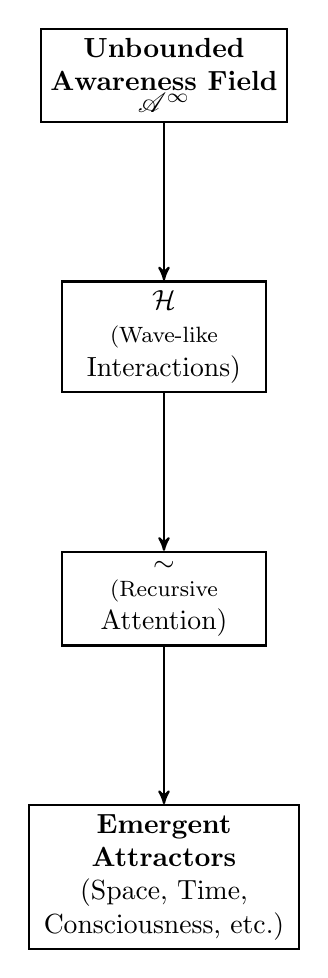
\begin{tikzpicture}[>=stealth',
    node distance=2.0cm,          % Vertical distance between nodes
    every node/.style={rectangle,
                       draw=black,
                       thick,
                       minimum width=2.6cm,  % Decrease/adjust to suit
                       minimum height=1.1cm, % likewise
                       align=center}]

  % Define nodes in a vertical stack:
  \node (Awareness) {\textbf{Unbounded}\\ \textbf{Awareness Field} \\[-4pt] $\mathscr{A}^\infty$};
  \node (WaveOps) [below=of Awareness] 
        {$\mathcal{H}$ \\ \footnotesize (Wave-like\\Interactions)};
  \node (Fold) [below=of WaveOps] 
        {\(\sim\) \\[-3pt] \footnotesize (Recursive\\Attention)};
  \node (Emergent) [below=of Fold, text width=3.2cm]
        {\textbf{Emergent}\\\textbf{Attractors}\\(Space, Time, Consciousness, etc.)};

  % Draw arrows from top to bottom
  \draw[->, thick] (Awareness) -- (WaveOps);
  \draw[->, thick] (WaveOps) -- (Fold);
  \draw[->, thick] (Fold) -- (Emergent);

\end{tikzpicture}
\caption{A simplified vertical schematic of the SRFT. 
Starting from the unbounded Awareness Field ($\mathscr{A}^\infty$), wave-like potentials ($\mathcal{H}$) 
are ``folded in'' via recursive Attention (\(\sim\)), resulting in emergent attractors 
(e.g., space, time, and subjective experience).}
\label{fig:seed-SRFT-schematic}
\end{figure}

\paragraph{Attention as an Intrinsic Drive.}
In standard usage, “attention” is seen as a cognitive act linked to an individual’s brain. 
In the SRFT framework, however, we propose that \(\sim\) should be interpreted as an \emph{intrinsic drive} 
or \emph{impetus} of \textbf{Attention} that arises \emph{within} the Awareness Field, rather than being imposed from outside. 
When \(\mathscr{A}^\infty \sim \mathscr{A}^\infty\) occurs, certain wave configurations become \emph{amplified} 
(higher probability), while others are \emph{damped} (lower probability). Through multiple “convolutions,” 
these amplified patterns stabilize into attractors, effectively generating time, space, and the other 
recognizable structures of experienced reality.

\paragraph{Connectivity Across Time}
Because the field is fundamentally unbounded, each emergent iteration---even after time appears---remains ``convoluted'' with the entire Awareness Field. In other words, while we speak of discrete stages of amplification or selection, these are never fully isolated. The recursive nature of Attention preserves a deep connectivity across what we label as ``past,'' ``present,'' and ``future'' moments.

\paragraph{Conceptual vs. Formal.}
We stress that the Seed Equation is \emph{not} a literal differential equation or PDE; it is a \emph{symbolic anchor} encapsulating how the SRFT envisions emergent multiplicities from an \textbf{unbounded Awareness Field}. As with \(\sin\) and \(\cos\) in wave equations, these wave-like interactions could be explored further through complexity science or advanced mathematics (e.g., \emph{fractional operators}) if one seeks more rigorous models. For our purposes, the equation underscores the idea that “folding in” is an \emph{intrinsic} dynamic of the Awareness Field, rather than an external force.

\subsection{Distinguishing Our Two Central Claims}

\noindent
In this paper, we emphasize two core claims central to the Self Referential Field Theory (SRFT):

\begin{description}
  \item[\textbf{(1) Ontological Claim: Unbounded Awareness Field}] 
  We posit an ``unbounded Awareness Field'' (\(\mathscr{A}^\infty\)) as the fundamental reality that underlies all phenomena. 
  This field is not confined by space or time, and serves as the metaphysical ``ground'' out of which both mind and matter arise.
  In contrast to purely materialist accounts, we treat consciousness (and even spacetime) as emergent \emph{within} this deeper field.

  \item[\textbf{(2) Mechanistic Principle: Recursive Attention}]
  We propose that ``recursive Attention'' (\(\sim\)) is the dynamic, \emph{self-referential} process by which latent potentials in the Awareness Field are selected, amplified, or dampened. 
  While we borrow the term ``attention'' from psychology and neuroscience, here it is meant more broadly: an iterative ``folding-in'' mechanism and intrinsic drive that gives rise to distinct phenomena (e.g., particles, thoughts, social structures). 
  From the emergent vantage (where time is already in play), this mechanism can be viewed as repeated cycles of ``focus'' or wave-like feedback that stabilize certain forms into coherence.
\end{description}

\noindent
Crucially, these two claims are \emph{distinct}: one describes \emph{what exists} at the most fundamental level (the Awareness Field), and the other \emph{how} that field manifests or differentiates (recursive Attention). By separating the ontological from the mechanistic, we avoid conflating the existence of a timeless substrate with the time-bound processes that give rise to stable phenomena.



\begin{table}[ht]
\centering
\caption{Contrasting the Ontological and Mechanistic Claims in the SRFT}
\label{tab:ontology-mechanism}
\begin{tabular}{p{3.2cm} p{5cm} p{5cm}}
\hline
 & \textbf{Unbounded Awareness Field} 
 & \textbf{Recursive Attention} \\ \hline
\textbf{Nature} 
 & Ontological (timeless foundation) 
 & Mechanistic (iterative selection within emergent time) \\
\textbf{Scope} 
 & Unlimited potentiality \newline (no spatial or temporal bounds)
 & Shaping discrete forms (particles, minds, societies) \\
\textbf{Key Role} 
 & Potentiality of all phenomena 
 & Feedback driver that crystallizes specific wave patterns \\
\textbf{Relation to Consciousness} 
 & Fundamental ground of experience 
 & Produces local subjective states via iterative focusing \\
\hline
\end{tabular}
\end{table}


\subsection{Emergence and Stable Attractors}
\label{subsubsec:emergence-attractors}

In this framework, \emph{Emergence} refers to how coherent, recognizable patterns (e.g., physical entities, mental states, social systems) crystallize from potentiality. Following insights from complexity science, we posit that certain self-reinforcing wave-like interactions form \emph{Stable Attractors} within the Awareness Field. An attractor, in dynamical systems language, is a set of states toward which a system evolves under iteration.

\paragraph{Iterative Formation of Attractors}
Strictly speaking, the notion of ``iteration'' is valid only once time is part of the emergent picture. From an \emph{emergent} standpoint, we say repeated cycles of \emph{Attention} reinforce particular wave-patterns, stabilizing them into persistent forms. Meanwhile, from the \emph{fundamental} (timeless) vantage, such ``iterations'' should be understood as conceptual placeholders for how unbounded potentiality differentiates into apparent sequences.


\subsubsection{Consciousness (in the SRFT Sense)}
\label{subsubsec:consciousness-SRFT}

Within the Self Referential Field Theory, we use the term \emph{consciousness} to denote 
the \emph{localized, phenomenal experience} that arises when \emph{recursive Attention} 
selectively amplifies certain wave-like potentials in the unbounded Awareness Field. 
While \textbf{Awareness} itself is treated as a universal \emph{ground} or 
\emph{field of potentiality}, consciousness \emph{appears} as a distinct “felt” state 
only when specific interactions---driven by attention---stabilize these potentials 
into coherent attractors (e.g., thoughts, perceptions, emotions). 

\paragraph{Key Distinctions.} 
\begin{itemize}
    \item \textbf{Awareness vs.\ Consciousness:} 
    In the SRFT, ``Awareness'' is the \emph{unbounded potentiality} encompassing all possible forms, while “consciousness” is one \emph{emergent 
    instantiation} of that potentiality, arising wherever recursive Attention organizes potentials into a \emph{felt} or \emph{experienced} state.
    
    \item \textbf{Local Vantage Points:} 
    Although the Awareness Field is universal and not tied to any single location, consciousness can manifest in \emph{localized attractors}, giving rise to the sense of an individual “subject” or “center” of experience. From the SRFT perspective, these local vantage points remain embedded in the unbounded field, even when they \emph{feel} discretely bounded.
    
    \item \textbf{Dynamics of “Folding In”:} 
    Consciousness arises moment-to-moment as \emph{recursive Attention} continually “folds in” on itself, selecting, reinforcing, or dissolving wave patterns. This iterative process underlies both the continuity of conscious experience (across time) and the capacity for sudden shifts in focus or state.
\end{itemize}

In essence, consciousness is not a standalone property that \emph{exists apart} from the Awareness Field; rather, it \emph{unfolds} from the \emph{self-referential} dynamics of attention within that field. By linking “consciousness” to the formation of stable, \emph{felt} attractors, the SRFT frames subjective experience as an \emph{emergent} yet \emph{integral} facet of a timeless and unbounded Awareness. 

\subsection{Timeless vs.\ Emergent Perspectives}

\noindent
A central aspect of the SRFT is that \emph{time itself} is viewed as emergent from a deeper, timeless ground. 
To clarify this, we distinguish two interpretive ``standpoints'':

\begin{description}
  \item[\textbf{Timeless / Ultimate Standpoint}] 
  From this vantage, the Awareness Field (\(\mathscr{A}^\infty\)) is \emph{not} embedded in space or time. 
  There is no ``before'' or ``after'' here---no linear chain of causes. 
  Instead, the Field simply \emph{is}, containing an infinite spectrum of potential forms.

  \item[\textbf{Emergent / Local Standpoint}] 
  Once stable attractors form, we perceive a sequential unfolding that we call ``time'' and a spatial framework that we call ``space.'' 
  Within this emergent view, we can describe \emph{recursive Attention} as iterating over states, ``selecting'' wave potentials at each step. 
  Thus, cause-and-effect, development, and the sense of history belong to this emergent domain, not to the ultimate.

\end{description}

\noindent
Hence, while it may sound paradoxical to speak of a ``timeless'' reality giving rise to iterative processes, this puzzle dissolves once we realize these are simply two complementary perspectives: one from within the emergent domain of phenomena, the other from the universal Field itself.

\paragraph{A Note on Zeno’s Paradox.}
Zeno’s paradoxes (e.g., Achilles and the Tortoise) famously highlight the apparent contradiction 
that arises when motion is subdivided into an infinite series of static intervals. 
From a SRFT standpoint, however, these paradoxes emerge only if one treats “time” 
as a pre-existing continuum that can be infinitely partitioned. By contrast, 
in our framework, \emph{time itself} emerges from each iteration or “fold” of recursive Attention. 
Thus, the field’s deeper, timeless ground does not suffer from the problem of infinite subdivisions; 
the appearance of consecutive “slices” of time is precisely what the field’s self-referential process 
generates, rather than a structure it must somehow traverse.

\subsection{Recursive Attention as a Generative Mechanism}
\label{subsec:recursive-attention}

\subsubsection{Conceptual Overview: Iterations That Create Time}
\emph{Recursive Attention} describes how the field of potentiality becomes self-referential: each ``act'' of Attention (again, understood in a metaphysical sense) brings forth a pattern from potential to manifestation. When these acts compound upon themselves, the emergent framework interprets them as ``iterations'' unfolding in time. Thus, the \emph{iterative process} is both \emph{the cause of} and \emph{contingent on} the emergent dimension of time.

\paragraph{Preserving Oneness Despite Differentiation}
Because these iterations occur within a single \textbf{unbounded} field, all newly crystallized forms (particles, thoughts, societies) remain interconnected through the shared \emph{Awareness Field}. The “convolution” of the field ensures that no attractor is ever truly isolated from the totality of Awareness; instead, each iteration folds back into the field, maintaining global coherence.

\subsubsection{Connections to Complexity Science}
\label{subsubsec:complexity-feedback}
In complexity theory, iterated functions and feedback loops can generate spontaneous order out of chaos. By analogy, in the SRFT, \emph{recursive Attention} is the underlying feedback principle. Once the emergent dimension of time is “in play,” we can describe how repeated cycles of selection/reinforcement yield stable attractors.

\paragraph{Maintaining Timeless Connectivity}
Nevertheless, we stress that from the ultimate standpoint, these cycles are not strictly temporal. The emergent vantage \emph{projects} an iterative structure onto the fundamental process, enabling a coherent narrative in which phenomena appear to develop or evolve. In that sense, the SRFT bridges a “timeless” field of potentiality and our everyday experience of linear time.

\subsubsection{Toward a Conceptual Formalism}
While a rigorous mathematical model is beyond scope here, we can outline one possible notation:
\[
A_{\tau+1} = \mathcal{F}\bigl(A_{\tau}, \,\alpha\bigr),
\]
where \(A_{\tau}\) is the apparent ``state'' of the Awareness Field at emergent time-step \(\tau\), \(\alpha\) indicates a parameter or direction of Attention, and \(\mathcal{F}\) is a recursive update function that either amplifies or dampens specific wave potentials. In truth, \(\tau\) itself arises from these iterative processes, making this formalism more of a \emph{conceptual mirror} than a literal depiction of a prior timeline.

\subsubsection{Consequences for Phenomenal Consciousness}
If local minds (e.g., human brains) are specialized amplifiers of certain wave-patterns, then \emph{phenomenal consciousness} reflects a distinct attractor class within the emergent time-bound universe. Neural feedback loops, from the SRFT perspective, harness the universal capacity of \emph{recursive Attention} but shape it into species-specific or individual-specific experiences. The felt unity of consciousness could thus be attributed to the field’s pervasive connectivity across all emergent states.

\paragraph{Unified Yet Differentiated}
Finally, while time and space allow the segmentation of experience, the original oneness of Awareness remains intact, preserving a deeper sense of continuity across all events. Hence, the SRFT posits that the emergence of differentiated phenomena (including time itself) does not sever them from the \textbf{unbounded} field but reconfigures them as locally stable attractors embedded in a globally connected reality.

\medskip

By specifying (1) a timeless field of potentiality, (2) space--time as emergent, and (3) \emph{recursive Attention} as the creative mechanism, we aim to offer a logically coherent picture of how the manifold forms of experience and reality arise. The following sections will revisit this framework through metaphorical illustrations, potential empirical implications, and anticipated criticisms, clarifying how \emph{iterations that create time} still remain enfolded within an \textbf{unbounded Awareness Field}.


\section{Convolution as the Core Mechanism}
\label{sec:convolution-core}

In this section, we deepen our focus on the \textbf{metaphorical ``convolution''} (sometimes symbolically 
denoted ``\(\sim\)''), which the Self Referential Field Theory (SRFT) treats as its \textbf{generative principle}. 
While previous sections mentioned how \(\mathscr{A}^\infty\)---the unbounded Awareness Field---undergoes 
a self-referential, iterative process, we now show in greater detail why this \textbf{convolution-like} 
operation is pivotal for explaining emergent time, the amplification or damping of phenomena, 
and the very essence of “what-it’s-like” subjective experience (the hard problem of consciousness).

\subsection{Defining the Metaphorical Convolution}
\label{subsec:convolution-definition}

We use the symbol ``\(\sim\)'' to denote this \emph{self-referential} “convolution” of the Awareness Field 
upon itself:
\[
  \mathscr{A}^\infty = \mathcal{H}(\mathscr{A}^\infty) \;\sim\; \mathscr{A}^\infty.
\]
Importantly, \(\sim\) is \textbf{not} a literal convolution in the signal-processing sense 
\(\int f(t-\tau)\,g(\tau)\,d\tau\). Instead, it is a \textbf{conceptual extension} meant to convey 
\emph{how} unbounded Awareness \emph{references} or “selects” its own latent potentials. Once time emerges, 
we interpret each “convolution” as an \emph{iteration}, but from the ultimate (timeless) vantage, 
iteration is purely conceptual.

\begin{itemize}
    \item \textbf{Why Call It ``Convolution''?} 
    We borrow the term to evoke a \emph{folding together} of potentials, 
    reminiscent of constructive or destructive interference in wave phenomena. 
    However, our usage encompasses \emph{self-reinforcing feedback} rather than 
    a strict mathematical transform.

    \item \textbf{Amplification vs.\ Damping:} 
    In each self-referential “fold,” some potentials are \emph{amplified} while others 
    are \emph{dampened}, analogous to how waves can reinforce or cancel. Yet here, an 
    \textbf{intrinsic feedback} (``Attention'') drives stable attractors 
    (Section~\ref{subsec:hard-problem-convolution}).
\end{itemize}

\paragraph{Central Claim.}
This metaphorical convolution is the crux of the SRFT: without it, we cannot explain 
\emph{how} an unbounded Awareness Field differentiates into the myriad forms (physical, 
mental, social) we observe within time and space. While a water-wave analogy 
helps visualize interference, \(\sim\) includes a \emph{self-referential} driver that 
sustains or dissolves patterns—unlike ordinary wave superposition, which typically disperses 
unless continuously driven.

\subsection{Convolution and the Emergence of Dimensions}
\label{subsec:emergent-dimensions}

A key implication of this \emph{feedback-based convolution} is that time, space, and other dimensions 
appear \emph{only} once it is viewed from the emergent standpoint:
\begin{itemize}
    \item \textbf{Time as Cumulative Convolution:} 
    Each “fold” of \(\mathscr{A}^\infty\) is retrospectively identified as a temporal ``step.'' 
    From the unbounded (timeless) perspective, there is no sequence; from \emph{inside} the 
    emergent system, these “convolutions” manifest as a continuous flow of time.

    \item \textbf{Fractal or Scale-Invariant Patterns:} 
    Iterative processes often yield fractals. If \(\mathscr{A}^\infty\) references itself 
    repeatedly across scales, we might see self-similar structures from subatomic 
    to cosmic levels. Some fractional PDE or Hilbert-space model might eventually formalize 
    these scale-dependent dynamics.
\end{itemize}

\subsubsection{Why This Is Not Just Wave Interference}
\label{subsec:not-just-wave-interference}

In standard physics, wave superposition generally disperses unless there is a resonant boundary 
or driving force. By contrast, the SRFT’s \emph{metaphorical convolution} (\(\sim\)) features 
\textbf{self-referential, selective feedback} (``Attention''), which actively sustains or 
damps certain patterns. Consequently, wave interference alone does not produce lasting form, 
whereas the SRFT posits that the field’s own self-awareness \emph{acts} like a boundary 
that continually “selects” which wave-configurations persist. This is why we do not merely 
speak of wave interference but rather a \emph{convolution-like} feedback in an unbounded 
Awareness Field.

\paragraph{Appearance of Discrete Forms and Particle-Like Splashes.}
Wave phenomena can appear to yield discrete “particles” (e.g., droplets from a splash, point-like 
detections in the quantum double-slit experiment). Similarly, in the SRFT’s conceptual frame, 
convolution can spawn localized “wave packets,” giving the inside observer a sense of isolated 
entities or particles. In consciousness terms, such “packets” may manifest as the felt sense 
of “Self” or “Isness,” where the underlying field momentarily “collapses” into a localized focus. 
Though reminiscent of wave interference, the crucial difference is the \emph{self-referential} 
aspect that guides which patterns stabilize across iterations.

\subsection{Why Metaphorical Convolution Drives Temporality}
\label{subsec:drives-temporality}

In mainstream physics, time is often taken as a fundamental parameter: 
a built-in dimension of spacetime along which processes evolve. By contrast, 
the Self Referential Field Theory (SRFT) proposes that \textbf{awareness precedes time}, 
and that \emph{metaphorical convolution} (the self-referential “folding” of the Awareness Field) 
\emph{generates} what we label as sequential or iterative experience. In other words, 
\textbf{time arises because the unbounded field repeatedly selects and re-selects wave configurations} 
across what, from the inside, appear as successive “moments.”

\paragraph{1. Timeless Vantage vs. Emergent Sequence}
From the ultimate vantage, the Awareness Field is \emph{unbounded} by either space or time. 
No external clock ticks; no “before” or “after” can be meaningfully assigned. 
However, once we adopt the \emph{emergent} vantage---the perspective where local forms 
and observers arise---each \emph{convolution} becomes an \emph{iteration} that “locks in” 
particular patterns. These iterations \emph{accumulate} into a chain of events 
that we experience as a flow of time.

\paragraph{2. Continuous Selection as a Temporal Driver}
In each self-referential “fold,” the Awareness Field effectively \emph{chooses} 
(whether actively or probabilistically) which latent potentials to amplify and which to damp. 
Because this selection process repeats indefinitely, the emergent viewpoint perceives 
an ongoing “stream.” Thus, time is not a pre-given container but rather 
\emph{the experiential signature of the field’s sustained feedback loops}.

\paragraph{3. The “Now” as a Convolution Snapshot}
A useful way to think about this is that each momentary “snapshot”---what we call “now”--- 
arises out of the field’s \emph{current} self-selection of wave configurations. 
As the field continually updates these selections, the “previous” arrangement fades 
into what we label “the past,” and the “future” remains a set of potentials yet to be 
convolved. Hence, the feeling of “moving through time” reflects 
\emph{the dynamic interplay} of consistent re-selection.

\paragraph{4. Bridging the Timeless and the Time-Bound}
Finally, the SRFT acknowledges a paradox: on one hand, from the fundamental level, 
\emph{no real clock} is ticking. On the other, from the emergent vantage, 
we observe a world in motion, cause-and-effect, and personal histories. 
The metaphorical convolution is precisely what bridges these vantage points: 
it \emph{generates} the inside sense of progression while remaining, in principle, 
beyond linear time. As such, the SRFT places “awareness first,” making spacetime 
and its apparent continuity outcomes of the field’s perpetual, self-reinforcing 
dynamics.

\paragraph{Implications for the Arrow of Time}
In standard physics, the arrow of time is often linked to entropy and thermodynamics. 
The SRFT suggests a complementary perspective in which \emph{time’s arrow} 
flows from the field’s iterative, selective nature: each “convolution step” 
produces a stable arrangement from among many possibilities. Though not necessarily 
in conflict with thermodynamic explanations, this approach reframes “time direction” 
as arising from a deeper, \emph{awareness-driven} process that picks certain 
wave patterns to persist.

\medskip

\noindent
\textbf{In summary}, by treating metaphorical convolution as an engine of iteration, 
we invert the usual hierarchy: time is not a prerequisite for awareness, 
but a byproduct of \emph{awareness} repeatedly selecting among its latent potentials. 
This shift has wide-reaching implications, inviting us to rethink the status of time 
as a merely emergent property of an inherently \emph{timeless} field.

\subsection{Convolution-Like Feedback in Non-Dual Practices}
\label{subsec:nondual-damping}

In many non-dual traditions (e.g., Advaita Vedanta, Dzogchen), advanced practitioners describe how 
focusing “awareness on awareness itself” can dissolve the sense of discrete objects, thoughts, 
or even time. Within the SRFT framework:

\begin{itemize}
    \item \textbf{Redirecting Attention:}
    When one \emph{withholds} attention from phenomena and refocuses it on the unbounded Awareness Field, 
    emergent forms lose “amplification” and may subside.

    \item \textbf{Damping (Destructive Interference):}
    If each form depends on continued convolution-like feedback, then directing awareness 
    to the \emph{field} itself reduces those wave-patterns. Phenomena briefly dissolve, 
    revealing a sense of “content-free” or “unbounded” awareness.
\end{itemize}

\paragraph{Experiential Correlates.}
Meditators often report emptiness, unity, or non-dual insight. Interpreted via the SRFT, these experiences 
reflect \textbf{shifting the target} of the field’s self-referencing away from specific forms 
and back toward the substrate. In essence, the symbolic operator \(\sim\) can amplify or damp forms, 
and advanced practice harnesses its “damping” path to encounter fundamental stillness.

\subsection{From Neural Assemblies to Social Systems}
\label{subsec:convolution-across-scales}

Although elaborated further in Section~\ref{sec:applications-extensions}, it is worth noting 
that this \emph{metaphorical convolution} can operate at multiple scales:

\begin{itemize}
    \item \textbf{Neural Dynamics:} Conscious perception arises when neural circuits repeatedly feed signals back on themselves, stabilizing into “global” attractors \cite{friston2010}. Moreover, research indicates that some meditative practices reduce Default Mode Network activity \cite{brewer2011}, interpreted here as “damping” self-focused feedback loops. 

    \item \textbf{Collective Phenomena:}
    Cultural myths or memes gain traction when enough individuals attend to them, becoming stable 
    in a shared “attention field.” Once collective focus shifts, these memes fade.
\end{itemize}

This cross-scale generality underscores a central aim of the SRFT: to show that \emph{self-referential feedback} 
within an Awareness Field can unify phenomena from the neural domain to social systems. 
Whether in cognition or culture, the principle of selecting, reinforcing, or damping patterns 
offers a cohesive lens on emergent complexity.

\medskip
\noindent
\textbf{Conclusion.}
Our metaphorical “convolution” (\(\sim\)) is the \textbf{heart} of the Self Referential Field Theory: 
it is the \emph{process} by which unity differentiates into multiplicity, by which “timeless potential” 
becomes “time-bound” iteration, and by which subjective interiority (the “hard problem”) emerges 
within a self-referential field. Contemplative traditions illustrate how \emph{damping} can be 
experienced first-person when attention reorients toward the \textbf{unbounded Awareness Field} 
rather than the objects it sustains. Having established the centrality of this conceptual 
\emph{convolution}, we turn next to broader applications, counterarguments, and future research directions.



\section{Harmonics as Wave-Like Interactions}
\label{sec:harmonics-core}

In the preceding section, we examined \emph{metaphorical convolution} (\(\sim\)) as the
self-referential ``folding in'' of the Awareness Field. This folding process shapes which latent potentials become amplified or dampened over
iterative cycles. Crucially, however, these potentials do not arise in a vacuum. They emerge
out of \(\mathcal{H}(\mathscr{A}^\infty)\), an operator we have thus far described simply as
representing ``wave-like'' or ``harmonic'' interactions in the unbounded Awareness Field.
In this section, we unpack the role of \(\mathcal{H}\) to show how \emph{harmonics}---in
the form of resonances, interference patterns, and stable modes---provide the essential
``content'' or ``geometry'' that \(\sim\) (convolution) operates upon. By clarifying
\(\mathcal{H}\), we more fully reveal how stable attractors and emergent features (space,
time, consciousness) could arise within the \textbf{Self Referential Field Theory (SRFT)}.

\subsection{Defining Harmonics in the SRFT Context}
\label{subsec:harmonics-definition}

We introduce \(\mathcal{H}(\mathscr{A}^\infty)\) as the set of \emph{wave-like interactions}
intrinsic to the unbounded Awareness Field \(\mathscr{A}^\infty\). In physical and mathematical
parlance, ``harmonics'' typically refers to oscillatory functions (e.g., sines, cosines) or
more abstract resonant modes (e.g., eigenfunctions of certain operators). While we do not
claim a one-to-one mapping with conventional physics, we analogize:
\begin{itemize}
    \item \textbf{Oscillatory Nature:} Just as simple harmonic motion recurs at characteristic
    frequencies, the Awareness Field may exhibit periodic structures or ``modes'' that can
    reinforce each other under certain conditions.
    \item \textbf{Resonant and Interferential Behavior:} Harmonics overlap, potentially causing
    constructive or destructive interference. In SRFT, certain wave-patterns stabilize into
    attractors when recursive Attention ``locks in'' or resonates with them.
    \item \textbf{Potential for Higher-Dimensional Waves:} While everyday experience
    confines us to 3D space + time, the SRFT posits an \emph{unbounded} field where these
    ``harmonic operators'' may extend far beyond typical 3D wave equations (e.g., involving
    fractional derivatives or higher-dimensional modes).
\end{itemize}

\paragraph{Interpretation.}
By calling these interactions ``harmonics,'' we highlight their capacity to form stable
patterns, much as musical instruments naturally produce discrete resonant tones.
Whereas conventional physics often treats wave equations in a pre-defined spacetime,
the SRFT views \emph{both} spacetime and wave phenomena as emerging within an unbounded
Awareness Field. This perspective broadens the traditional notion of harmonics to
include the possibility that \emph{space} and \emph{time} themselves result from stable
wave-like attractors, rather than being pre-existing containers for the waves.

\subsection{Harmonic Resonances and the Emergence of Stability}
\label{subsec:harmonic-resonances}

Resonance occurs when wave-like processes align in frequency or phase, creating amplified,
self-reinforcing patterns. In classical mechanics, a string fixed at two ends sustains
discrete standing waves at particular frequencies (harmonics). These modes are stable
solutions of the wave equation. Analogously, within the SRFT framework:
\begin{itemize}
    \item The \emph{Awareness Field} (\(\mathscr{A}^\infty\)) can be viewed as having
    \textbf{infinitely many} latent modes. 
    \item \(\mathcal{H}\) is the \emph{operator} encoding how these modes interact,
    potentially leading to resonant alignments (constructive interference) or cancellations
    (destructive interference).
    \item The \emph{convolution-like feedback} (\(\sim\)) repeatedly “folds in” the current
    state of the field, selecting or amplifying resonant modes. This iterative feedback
    can lock certain modes into stable attractors, effectively “pinning down” recognizable
    forms (e.g., particles, mental states, or social structures).
\end{itemize}

\paragraph{Why Resonance Matters.}
In dynamical systems, a resonance can cause a pattern to persist or even grow in amplitude
once established. Similarly, \emph{recursive Attention} might continually energize certain
harmonic modes of \(\mathcal{H}\), leading to stable, emergent phenomena across multiple
time-scales. Examples might include:
\begin{enumerate}
    \item \textbf{Neural Oscillations:} Brain rhythms (e.g., gamma frequencies) persist
    when neural circuits reinforce one another, akin to standing waves in the cerebral
    cortex \cite{friston2010, tononi2008}.
    \item \textbf{Social Norms:} Collective “attention fields” can align around certain
    ideas or memes, making them resonate and persist longer in cultural discourse.
    \item \textbf{Physical Structures:} From atoms to galaxies, repeated oscillatory
    processes lock into stable attractors, forming the building blocks of matter.
\end{enumerate}

\subsection{Comparisons with Standard Wave Interference}
\label{subsec:harmonics-vs-wave-interference}

A question might arise: ``Isn’t this just standard wave superposition? Why call it
\(\mathcal{H}\)?'' The key differences are:

\begin{itemize}
    \item \textbf{Intrinsic Operator vs. External Waves:}
    In typical physics, waves propagate in a pre-existing metric space (e.g., 3D
    Euclidean space, Minkowski spacetime). In SRFT, \emph{space} itself is an
    \textbf{emergent} attractor. Thus, \(\mathcal{H}\) functions as an \emph{intrinsic}
    operator within \(\mathscr{A}^\infty\), not simply a wave equation embedded in
    external spacetime.
    \item \textbf{Self-Referential Feedback:}
    Standard wave interference often disperses unless there’s a boundary or driving force.
    Here, \emph{recursive Attention} acts like a boundary+driver \emph{within} the field,
    sustaining or damping certain harmonic modes over “iterations.”
    \item \textbf{Connection to Convolution:}
    While wave superposition typically involves linear addition of amplitudes, SRFT’s
    “folding in” can be seen as a \emph{nonlinear} or self-referential convolution. This
    means the amplitude of each mode can change nonlinearly in response to the field’s
    overall state, allowing for \emph{adaptive} stabilization of certain modes and
    suppression of others.
\end{itemize}

\subsection{Linking \texorpdfstring{$\mathcal{H}$}{H} to Convolution \texorpdfstring{$\sim$}{\textasciitilde}}
\label{subsec:h-and-convolution}

To appreciate how \(\mathcal{H}\) and \(\sim\) work together, recall the Seed Equation:
\[
\mathscr{A}^\infty
\;=\;
\mathcal{H}(\mathscr{A}^\infty)
\;\sim\;
\mathscr{A}^\infty.
\]
Here, \(\mathcal{H}\) captures the \emph{wave-like basis} of potential patterns in the
Awareness Field, while \(\sim\) denotes the self-referential ``folding'' driven by recursive
Attention. Thus:
\begin{enumerate}
    \item \(\mathcal{H}(\mathscr{A}^\infty)\) reveals the \textbf{harmonic possibilities}
    latent in the field.
    \item \(\sim\) (convolution) \textbf{selects and refines} these possibilities by
    repeatedly referencing the field against itself. Over what we call ``iterations,''
    certain harmonic modes become \emph{stable attractors}.
\end{enumerate}

In simpler wave systems, stable standing waves form when boundary conditions reflect the
wave back upon itself in-phase. By analogy, \(\sim\) is the process of reflecting the
field’s potential \emph{back upon itself}, aligning phases for certain frequencies and
manifesting stable phenomena. If \(\mathcal{H}\) is the ``theater'' in which wave-forms
unfold, \(\sim\) is the script ensuring that certain performances (patterns) recur
night after night, becoming \emph{realities} within emergent time and space.

\subsection{Implications Across Scales and Future Directions}
\label{subsec:harmonics-implications}

By foregrounding \(\mathcal{H}\) as a harmonic or wave-like operator, the SRFT gains a
richer explanatory scope:

\begin{itemize}
    \item \textbf{Neural Oscillations and Conscious States:} Many theories of consciousness
    emphasize the importance of neural rhythms \cite{tononi2008,friston2010}. Casting
    \(\mathcal{H}\) in terms of resonant modes could unify standard neural oscillation
    models with the SRFT’s claim that an unbounded Awareness Field underlies these wave
    patterns. Recursively folded attention might ``lock in'' specific synchronization
    patterns, yielding the subjective unity of consciousness.
    \item \textbf{Collective Attention and Social Memes:} Harmonic patterns need not be
    confined to physical or neural domains; group attention might produce wave-like
    cycles (e.g., repeated news cycles, meme virality). \(\mathcal{H}\) offers a lens
    for seeing how certain cultural “frequencies” or ideas resonate collectively, forming
    stable attractors in social space.
    \item \textbf{Physical Structures at Cosmic Scales:} In cosmology, standing-wave
    patterns have been linked to cosmic microwave background fluctuations or galaxy
    distribution filaments. If \(\mathscr{A}^\infty\) extends beyond standard spacetime,
    \(\mathcal{H}\) may symbolize deeper resonances that underlie fractal cosmic webs,
    black-hole information puzzles, or other frontier topics in theoretical physics.
    \item \textbf{Mathematical Formalization:} Possible next steps include modeling
    \(\mathcal{H}\) as a fractional-dimension operator or using Fourier-like expansions
    in multi-scale PDEs. Investigating how \(\sim\) (convolution) selects certain
    harmonics over many “iterations” can provide clues to how fractal or scale-invariant
    patterns materialize. 
\end{itemize}

\paragraph{Recap and Synthesis.}
Harmonics (\(\mathcal{H}\)) and convolution (\(\sim\)) operate in tandem to differentiate
the unbounded Awareness Field \(\mathscr{A}^\infty\) into coherent forms. Where
\emph{convolution} explains the iterative, self-referential \emph{process}, harmonics
explain the \emph{content} or \emph{structure} of potential wave-forms available to be
selected. Through this interplay, stable attractors---whether neural, social, or cosmic---arise
naturally, illustrating how unity can differentiate into multiplicity without losing its
fundamental connectedness.

\medskip
\noindent
\textbf{Conclusion of the Harmonics Deep Dive.} 
By illuminating the role of \(\mathcal{H}\) in generating wave-like potentials, we extend
the SRFT beyond a simple “folding in” metaphor. Harmonic interactions provide the scaffolding
of resonant modes, while recursive Attention “folds” these modes into stable, persistent
patterns. Together, \(\mathcal{H}\) and \(\sim\) form the heart of the Seed Equation,
shedding light on how an \emph{unbounded Awareness Field} might manifest as the diverse,
time-bound reality we experience.

\section{Emergent Features: Patterns and Stable Attractors}
\label{sec:emergent-features}

A key question arising from the discussion of \(\mathcal{H}(\mathscr{A}^\infty)\) (harmonic,
wave-like interactions) and \(\sim\) (convolution-like folding in) is:
\emph{``Yes, but \textbf{how} do novel or stable patterns actually form?''}
This section addresses that question head-on, showing how recursive Attention
transforms an unbounded reservoir of wave potentials into concrete, enduring
phenomena. Put simply: stable attractors---the \emph{patterns} we identify as
physical structures, mental states, and social constructs---arise when certain
wave configurations are repeatedly \emph{selected} or \emph{reinforced} within
the unbounded Awareness Field.

\subsection{From Latent Potentials to Emergent Forms}
\label{subsec:latent-to-emergent}

While Sections~\ref{sec:convolution-core} and \ref{sec:harmonics-core} introduced
\(\sim\) (convolution-like feedback) and \(\mathcal{H}\) (harmonic processes),
the specific \emph{outcome} of these interactions requires a clear statement:
\begin{enumerate}
    \item \textbf{Wave-Like Potentials (\(\mathcal{H}\)):} The unbounded Awareness Field,
    denoted \(\mathscr{A}^\infty\), contains infinitely many \emph{latent modes}---akin
    to potential waveforms. These modes can \emph{interfere} (constructively or
    destructively), forming complex interference patterns.

    \item \textbf{Recursive Convolution (\(\sim\)):} This is the \emph{self-referential
    folding} (focused attention) of the Awareness Field back onto itself. Each ``fold'' amplifies or
    diminishes particular wave-modes, depending on how they resonate with (or cancel)
    existing patterns.

    \item \textbf{Iteration and Selection:} Over multiple ``folds'' (from the emergent
    vantage, we call these \emph{iterations}), certain wave configurations become
    increasingly \emph{probable} or \emph{salient}, stabilizing into \textbf{attractors}.
    Others fade.
\end{enumerate}
Taken together, \(\mathcal{H}\) sets the \emph{structure} of possible interactions,
while \(\sim\) (convolution) drives an iterative \emph{selection} process, locking
in patterns that continually reinforce themselves in the Awareness Field.

\subsection{Stable Attractors: Coherence Amid Infinite Possibility}
\label{subsec:stable-attractors}

\paragraph{Attractors in Dynamical Systems.}
In complexity science, an \emph{attractor} is a set of states a system converges
to under repeated iteration---for example, a pendulum that settles into a
predictable swing pattern. In the SRFT, we apply this concept to the unbounded
Awareness Field:
\begin{itemize}
    \item \emph{Stable attractors} form when recursive Attention \textbf{consistently}
    amplifies certain harmonic modes. Over \emph{emergent time}, these modes coalesce
    into coherent structures (e.g., persistent wave patterns, neural oscillations,
    social memes).
    \item If no resonance is established, wave interference may remain chaotic or
    transitory, creating fleeting patterns (like ripples that dissipate).
\end{itemize}

% ===============================================
% Insert where you first discuss wave or ripple metaphors
% ===============================================

\subsubsection{Clarifying the Wave Metaphor}

\noindent
While we frequently invoke ``wave'' language (e.g., interference, harmonics, standing waves) to illustrate how phenomena can emerge or dissolve, 
it is important to note that we are not necessarily claiming a strict \emph{physical} wave equation in three-dimensional space.
Rather, ``wave'' here encompasses any oscillatory or resonant pattern within the Awareness Field that can exhibit interference-like behavior.
The term ``wave'' thus serves as an \emph{analogy} for constructive and destructive interactions among latent potentials.

\begin{quote}
\textit{In principle, one could attempt to formalize these processes using fractional partial differential equations or iterative maps in a generalized space (not necessarily 3D). 
Such a model would treat ``convolution-like feedback'' as a selection operator that reinforces certain wave modes, somewhat analogous to stable standing waves in classical physics.
However, we leave the detailed PDE approach to future theoretical work (see Section~\ref{sec:future-work} for possible directions).}
\end{quote}


\paragraph{Emergence of Novelty.}
Even though many dynamical systems eventually settle into familiar attractors, new
patterns can arise when \emph{perturbations} or fresh “folds” re-inject energy into
the system. In the SRFT framework:
\begin{itemize}
    \item A spike of focused Attention can trigger a “wave splash,” momentarily
    disrupting stable attractors and flinging out new droplets or wavelets.
    \item If those droplets resonate (constructively) with existing modes, they may
    seed \emph{novel} attractors. Thus, novelty and dissolution operate hand-in-hand,
    continually updating the emergent tapestry of \(\mathscr{A}^\infty\).
\end{itemize}

\subsection{Iterative Path: From Timeless Potential to Time-Bound Phenomena}
\label{subsec:iterative-path}

\paragraph{Timeless Vantage vs.\ Emergent Sequence.}
Recalling Section~\ref{sec:core-foundations}, the SRFT posits a \emph{timeless} (or
“ultimate”) vantage in which \(\mathscr{A}^\infty\) simply \emph{is}, prior to any
space--time. However, once we adopt the \emph{emergent} vantage:
\begin{enumerate}
    \item Each act of ``self-folding'' (convolution) is viewed as a \emph{step in time}.
    \item These steps accumulate into an apparent \emph{temporal sequence}, yielding
    stable attractors that we recognize as persistent forms and events.
\end{enumerate}
Hence, \emph{time} itself is an outgrowth of repeated \emph{feedback selection}
in the Awareness Field. Novel patterns or stable attractors \emph{become} the
entities we catalog as “objects,” “organisms,” or “societies”---all nested within
the larger web of wave-like interactions.

\subsection{Damping, Dissolution, and the Ongoing Dance of Emergence}
\label{subsec:damping-dissolution}

\paragraph{Not All Waves Persist.}
An equally important aspect of emergent phenomena is the \emph{dissolution} of
patterns. In wave analogies, not every ripple remains stable; many simply cancel
out. Likewise, the SRFT suggests that some thought-forms, physical structures, or
social memes fail to secure \emph{sustained} attention and thus fade:
\begin{itemize}
    \item \textbf{Damping}: When recursive Attention \emph{withdraws} from a pattern,
    destructive interference rises. The wave-form loses amplitude and dissolves back
    into the broader field.
    \item \textbf{Reinjection of Energy}: Occasionally, a “crash” or disruptor can
    create droplet-like spinoffs, injecting new wavelets that might form \emph{fresh}
    attractors if they find resonance.
\end{itemize}
This cycle of \textbf{emergence} (stabilization) and \textbf{dissolution}
(damping) ensures the Awareness Field never “freezes.” It remains dynamic,
potentially giving rise to continuous innovation and diversity of forms.

\subsection{Cross-Scale Examples of Emergent Attractors}
\label{subsec:cross-scale-attractors}

Even though the \emph{mechanism} (recursive Attention) remains the same, the
\emph{manifestation} of stable attractors spans multiple scales:

\begin{itemize}
    \item \textbf{Particle-Like Forms:}  
    In physics, wave--particle duality allows wavefunctions to appear as “point-like”
    detections. Within the SRFT lens, these local “collapses” can be viewed as stable
    attractors supported by repeated self-referential attention in the field, giving
    matter its seemingly discrete nature.

    \item \textbf{Neural Oscillations and Cognition:}  
    Neural circuits exhibit rhythmic patterns (e.g., gamma oscillations) that can lock
    in or shift, shaping conscious states. Here, stable attractors correspond to
    \emph{neural synchrony}, potentially revealing how subjective experience forms
    from wave-like coordination.

    \item \textbf{Social Norms or Memes:}  
    On a collective scale, an idea or “meme” can become a stable attractor if enough
    shared attention converges on it (e.g., viral trends, cultural beliefs). Over
    \emph{emergent} time, it persists until attention wanes or new disruptors appear.

    \item \textbf{Fractal, Scale-Invariant Patterns:}  
    As discussed in Section~\ref{subsec:fractal-patterns}, iterative folding can produce
    fractal or self-similar forms across scales, from leaf venation to large-scale cosmic
    filaments. These robust patterns exemplify stable attractors repeated in multiple
    domains.
\end{itemize}

\subsection{Answering the Core Question: ``How Do Novel or Stable Patterns Form?''}
\label{subsec:how-they-form}

Bringing these threads together, the SRFT’s reply to “\emph{How do new phenomena
\textbf{actually} emerge?}” can be summarized in three steps:

\begin{enumerate}
    \item \textbf{Open Potential:} The unbounded Awareness Field, \(\mathscr{A}^\infty\),
    contains infinite \emph{latent} wave-like possibilities. No single outcome is fixed
    \emph{a priori}.
    \item \textbf{Recursive Selection:} Through the convolution-like operation
    (\(\sim\)) of \emph{recursive Attention}, the system “selects” wave configurations
    that \emph{resonate} with existing patterns. Constructive interference amplifies
    them, destructive interference dampens others.
    \item \textbf{Stable Attractors (Emergence)}: Repetitive “folds” fix or anchor
    certain patterns as stable attractors, while less-supported possibilities dissolve.
    Over emergent time, these attractors manifest as physical, cognitive, or social
    phenomena. Shifts in attention or perturbations inject novelty, seeding new or
    modified attractors.
\end{enumerate}

Hence, stable patterns---from an electron’s localization to a cultural movement---are
\emph{not} static objects \emph{in} a pre-given universe but dynamic, wave-based
attractors \emph{co-created} by ongoing self-referential folding in an \textbf{unbounded
Awareness Field}.

\subsection{Implications for the Broader Theory}
\label{subsec:emergent-implications}

By laying out how novelty arises and why certain phenomena \emph{persist}, this
section clarifies the backbone of the SRFT:
\begin{itemize}
    \item \textbf{Bridging Metaphysics and Complexity Science:} Non-dual philosophies
    often speak of a single source unfolding into many forms, yet rarely specify a
    \emph{mechanistic driver}. Complexity science models attractors and feedback loops,
    yet typically assumes a physical substrate. The SRFT combines both standpoints,
    attributing emergent order to the self-referential \textbf{Awareness Field}.
    \item \textbf{Time as Emergent Outcome:} Because stable attractors only form via
    iterative selection, \emph{time} itself is a \emph{product} of this perpetual
    “folding in.” Consequently, every persistent phenomenon arises via the \emph{flow}
    of emergent time.
    \item \textbf{Cross-Scale Unity:} From subatomic particles to collective societies,
    the same principle of wave resonance and folding can unify disparate levels of
    analysis---a continuity that purely reductionist models often struggle to maintain.
\end{itemize}

Overall, by specifying \textbf{how} wave-like potentials become stable, recognizable
patterns, we show that the step from “unbounded potentiality” to “discrete entities”
need not be a mysterious leap. In the SRFT framework, the \emph{selection} process
driven by recursive Attention and wave harmonics provides a conceptual route
for emergent features to arise and persist.

\medskip
\noindent
\textbf{In Conclusion.}  
Novel or stable patterns form when the \emph{unbounded Awareness Field} iteratively
folds upon itself, \emph{amplifying} certain harmonic modes into long-lived attractors.
These attractors---whether subatomic, psychological, or cultural---are never wholly
detached from the Awareness Field that sustains them. Rather, they reflect localized
regions of resonance, continually shaped (and reshaped) by the ongoing dance of
attention, interference, and feedback. This dynamic view of emergence helps unify
the multiplicity of forms we encounter with the underlying oneness hypothesized
by the SRFT.

In short, reality—at least as we perceive it—coalesces around those wave potentials that the unbounded field repeatedly \emph{focuses on}, thereby solidifying them into stable forms.

\section{Key Debates in Consciousness and Reality}
\label{sec:key-debates}

In the preceding sections, we have seen how an \emph{unbounded Awareness Field},
shaped by recursive Attention and wave-like harmonics, could generate stable
attractors ranging from physical particles to social norms. We now turn to two
deep philosophical and scientific puzzles: the \emph{Hard Problem of Consciousness}
and the \emph{challenge of Agency \& Free Will}. Though distinct, both hinge on
the question of \emph{subjectivity}—how reality “feels” from the inside and
whether (or how) a feeling subject has genuine volitional power.



\subsection{The Hard Problem of Consciousness: Stable Attractors and the ``What-It’s-Like'' Dimension}
\label{subsec:hard-problem-convolution}

A longstanding challenge in consciousness studies is explaining the subjective \emph{what-it’s-like} 
dimension (the “hard problem” \cite{chalmers1995}). Physicalist or functionalist models 
show \emph{how} systems process information but not \emph{why} an \emph{inner feel} arises \cite{nagel1974bat}. 
In the SRFT, we posit that this \textbf{convolution-like feedback} intrinsically \emph{generates} 
felt interiority whenever the field references itself.

\paragraph{SRFT’s Non-Dual Reframing.}
At the heart of the SRFT is an \emph{unbounded Awareness Field} (\(\mathscr{A}^\infty\)), 
treated as ontologically primary rather than a byproduct of matter. Physical laws, spacetime, 
and even discrete minds emerge as \textbf{stable attractors} within this field. 
Hence, \emph{subjective experience} is not an afterthought but a \emph{natural expression} 
of the field’s self-referencing.

\paragraph{Self-Referential Spark.}
Each “convolution” of \(\mathscr{A}^\infty\) upon itself is the field \emph{knowing} itself. 
Instead of “How does matter produce mind?” the SRFT reverses the question to “How does universal 
awareness differentiate into matter, and retain an intrinsic feel whenever it ‘folds’ back 
onto itself?” From the \emph{inside}, this self-referencing manifests as “isness.”

\paragraph{Reframing the Explanatory Gap.}
By starting with awareness, we shift the “hard problem” from \emph{combination} (how inert matter 
aggregates into mind) to \emph{differentiation} (how a single field spawns multiple subjects). 
Consciousness thus becomes one \textbf{stable attractor} among many in an infinite-dimensional 
awareness-based reality.

\paragraph{Disclaimers and Caveats.}
\begin{itemize}
    \item \textbf{Philosophical, Not Strictly Empirical.} 
    While inspired by non-dual traditions, the SRFT is a conceptual lens rather than a laboratory theory. 
    We treat subjective experience as the field’s self-knowing aspect, not an emergent epiphenomenon.

    \item \textbf{Falsifiability.}
    Some predictions (e.g., fractal scaling in cognition) may be testable (Section~\ref{subsec:testable-claims}). 
    But the claim that “\(\mathscr{A}^\infty\) referencing itself yields felt interiority” remains metaphysical.

    \item \textbf{Call for Interdisciplinary Development.}
    Future models (e.g., fractional PDEs, agent-based simulations) might approximate self-referential wave dynamics 
    (Section~\ref{subsec:seed-equation}). Whether they reproduce “isness” is largely philosophical, 
    but bridging phenomenology and dynamical fields remains an intriguing prospect.
\end{itemize}

\paragraph{Practical Implications.}
\begin{enumerate}
    \item \textbf{Neuroscience/Phenomenology:} 
    Studies of meditation or “\emph{attention to attention}” could explore 
    neural/experiential markers correlated with heightened qualia.

    \item \textbf{Transpersonal Practices:} 
    Many traditions teach turning awareness onto itself to intensify the sense of being. 
    The SRFT interprets this as revealing the field’s stable attractor states.

    \item \textbf{Philosophical Engagement:} 
    Focusing on “How does awareness differentiate?” opens fresh debates 
    in panpsychism, non-dualism, and self-referential systems.

    \item \textbf{Frontiers in AI:}
    If AGI models incorporate loops of “\emph{attention to attention},” 
    might they exhibit a proto-“isness”? This remains speculative yet suggestive.
\end{enumerate}

\paragraph{Summary.}
In short, the SRFT \emph{relocates} rather than \emph{resolves} the hard problem: 
an inherently self-aware field differentiates into localized forms, accounting for 
why consciousness arises as an intrinsic dimension of \textbf{convolution-like feedback}. 
Though speculative, this view may inspire new lines of inquiry that merge subjectivity 
with dynamical models of reality.


\subsection{Agency and Free Will: The Emergent Sense of ``Doer-Ship''}
\label{sec:agency-freewill}

While the previous discussion focused on the \emph{qualitative} dimension of experience
(\emph{why} consciousness feels like something from the inside), the question of
\emph{agency} and \emph{free will} raises an additional layer: \emph{how} and \emph{why}
does an experiencing entity come to perceive itself as an \textbf{agent} capable of
intending or causing action? 

In modern philosophy, \emph{agency} often refers to the capacity of an individual
or system to initiate events intentionally \cite{shoemaker2003agency,metzinger2003subject}. Discussions of \emph{free will} pose the
deeper question: does this sense of control correspond to an actual power to choose,
or is it an illusion arising from deterministic processes \cite{wegner2002}?
In conventional neuroscience and psychology, agency is frequently modeled as the interplay
between \emph{motor commands}, \emph{internal predictions}, and \emph{proprioceptive} or
\emph{sensory} feedback \cite{frith2012action}, while metaphysical debates continue over
whether volition itself is \emph{causally efficacious} or simply an epiphenomenon
\cite{whitehead1929process}.

\paragraph{SRFT Perspective: Emergent Doer-Ship via Recursive Attention}
\label{subsec:SRFT-agency-perspective}

Within the Self Referential Field Theory (SRFT), we propose that the \emph{unbounded
Awareness Field} (\(\mathscr{A}^\infty\)) does not merely \emph{know}, but---through
\emph{recursive Attention}---also \emph{selects} and \emph{amplifies} potentials in a way
that can look, from the inside, like \textbf{willful action}. Concretely:
\begin{enumerate}
    \item \textbf{Field-Like Foundation:} From the ultimate (timeless) standpoint,
    all potentials for form and action lie within the \emph{unbounded Awareness Field}.

    \item \textbf{Self-Referential Selection:} The \emph{convolution} (\(\sim\)) of
    this field upon itself produces local \emph{loops} in which certain patterns
    reinforce. When these loops specifically track \emph{intentional states} or
    “commands” (e.g., forming a mental intention to move a hand), they become stable
    attractors for \emph{directed} activity.

    \item \textbf{Emergent Subject--Object Split:} As the Awareness Field partitions
    itself into localized vantage points (the “subject” of experience) and outward
    objects or tasks (the “object” of intention), \emph{agency} emerges as the subjective
    signature of \textbf{initiating change}. In effect, a specialized \emph{feedback loop}
    arises, labeling certain wave-patterns “\emph{my actions}” and identifying others as
    “\emph{external}.”
\end{enumerate}

\noindent
Hence, from the local vantage, it \emph{feels} like “I am doing this.” Yet from the
SRFT’s universal perspective, agency is an \emph{attractor state} in which the
\emph{unbounded Field} briefly \emph{localizes} around a cluster of potentials, giving
rise to the strong sense of willful, purposeful movement or thought.

\paragraph{Free Will vs.\ Determinism: Rethinking the Debate}
\label{subsec:freewill-debate}

Since time and space are \emph{emergent} in the SRFT, the usual debate between free will
and determinism shifts significantly:
\begin{itemize}
    \item \textbf{Emergent Time and Choice Points:} If time itself arises from repeated
    “folding,” then each new “moment” in the \emph{emergent vantage} is literally the
    \emph{result} of the field’s ongoing selections. From this perspective, we can
    interpret \emph{choice} as an actual \emph{inflection point} in the field’s next
    self-iteration, rather than a deterministic chain locked in from a past timeline.

    \item \textbf{Partial Illusion, Partial Efficacy:} The SRFT can accommodate both:
    \begin{enumerate}
        \item \emph{Illusion} in the sense that the local “self” is not separate from
        the universal Field, so “my action” is also “the field unfolding” \cite{wegner2002,metzinger2003subject}.
        \item \emph{Causal Efficacy} in the sense that focusing attention on specific
        potentials indeed \emph{amplifies} them, altering subsequent “slices” of
        emergent reality \cite{whitehead1929process}.
    \end{enumerate}
    In this sense, \emph{agency} is neither purely illusory nor purely absolute; it is
    one of the stable patterns by which the \textbf{field enacts} local changes through
    the lens of an apparent individual.

    \item \textbf{Revisiting Determinism:} While physical laws may appear deterministic
    in certain scales or contexts, the \emph{SRFT approach} suggests a deeper reality in
    which self-referential selection is always at play, thus leaving “room” for genuine
    novelty or choice. This may align with certain interpretations of process philosophy
    or non-dual traditions \cite{whitehead1929process} where “God or Awareness acts
    through every being” rather than each being acting \emph{independently}.
\end{itemize}

\paragraph{Agency as a Specialized Feedback Loop}
\label{subsec:agency-feedback-loop}

Drawing upon the concept of \emph{attractors} from Sections~\ref{sec:emergent-features}
and \ref{sec:convolution-core}:
\begin{enumerate}
    \item \textbf{Attentional Lock-In:} The sense of “I intend \textit{this} motion”
    arises when repeated “folds” (convolution steps) \emph{lock in} a wave pattern
    related to \emph{motor planning} or \emph{cognitive impetus}, anchoring it in the
    local vantage as “my action.”

    \item \textbf{Correlating with Neural Circuits:} In neuroscience, certain fronto-parietal
    loops or sensorimotor networks strongly correlate with volitional acts
    \cite{frith2012action}. The SRFT reinterprets these neural processes as
    \emph{localized attractors} that the Awareness Field “energizes” through
    \emph{recursive Attention}. Hence, from an emergent perspective, volitional neural
    patterns are amplified waveforms in the field, coalescing around an
    \emph{intended outcome}.

    \item \textbf{Self-Tagging of Control:} A hallmark of agency is that the subject
    \emph{attributes} the resulting movement or effect to itself. This “sense of ownership”
    is another wave pattern, \emph{tagging} certain signals (motor or sensory) as “mine”
    rather than “external.” The \emph{selection} mechanism is thus not just about
    physical movement but about labeling experiences as \emph{internally caused}.
\end{enumerate}

\noindent
In simpler terms, \emph{agency} emerges when the field organizes local wave modes
(physical or mental) into a cohesive \emph{“I did that”} narrative. While neural or
psychological models describe the \emph{functional} aspects, the SRFT offers an
\emph{ontological} substrate: all these loops exist within—and are guided by—the
unbounded, self-referential Awareness Field.

\paragraph{Implications for Coaching and Personal Development}
\label{subsec:agency-coaching}

From a practical standpoint, seeing agency as a \emph{stable attractor} shaped by
attention has implications for personal growth, therapy, and coaching contexts:
\begin{itemize}
    \item \textbf{Shifting the Attractor Basin:} If attention is the driver, then
    altering habitual patterns of focus can change one’s perceived level of control.
    Practices like mindfulness, self-inquiry, or cognitive reframing may “re-tune” the
    loops that yield the feeling of efficacy or hopelessness
    \cite{shapiro2006mindfulness}.

    \item \textbf{Dissolving or Strengthening the Sense of Doer-Ship:} Some contemplative
    traditions teach letting go of the “I am the doer” stance, revealing a more
    universal flow of action \cite{ramacandra1923upanishads}. Others reinforce self-efficacy
    for empowerment. Both reflect different modes of \emph{folding} the Field,
    re-labelling who or what “initiates” movement.

    \item \textbf{Relevance to Behavioral Change:} Many coaching frameworks focus on
    “choice architecture” or “attention management.” Under the SRFT lens, these methods
    reorient the \emph{self-reinforcing loops} that define one’s sense of choice. The
    more one trains attention on productive or growth-oriented potentials, the more
    those potentials become stable attractors for agency
    \cite{baumeister2008freewill}.
\end{itemize}

\paragraph{Future Directions: Agency Research Under the SRFT Lens}
\label{subsec:agency-future-work}

Much like the \emph{Hard Problem}, agency remains an open arena for empirical and
conceptual exploration. Potential next steps include:
\begin{itemize}
    \item \textbf{Neurophenomenological Studies:} Pair neural imaging of voluntary actions
    with micro-phenomenological interviews to see if changes in attention directly
    modulate the \emph{felt} sense of “I am doing this” \cite{petitmengin2006}.
    \item \textbf{Agent-Based Models:} Construct simulations where “agent-like” subsystems
    receive the capacity to select wave patterns. Observe if coherent “agency” emerges
    whenever certain feedback loops become self-tagged as “my action.”
    \item \textbf{Philosophical Analysis of Free Will and Determinism:} Engage with
    analytic debates to refine how the SRFT’s emergent-time approach might reconcile
    top-down selection (via attention) with bottom-up lawful dynamics (physical or
    neural) \cite{shoemaker2003agency,whitehead1929process}.
\end{itemize}

\noindent
Overall, \emph{agency} and \emph{free will} in the SRFT are interpreted as a
specialized mode of self-referential \emph{folding}, wherein localized wave-patterns
take on a \textbf{doer-ship signature}. Rather than a fixed or illusory phenomenon,
agency emerges as an \textbf{attractor state} shaped by repeated selection—a notion
that we hope can inspire new theoretical and empirical avenues in both philosophy
and science.

\subsubsection{Concluding Thoughts on Agency}
\label{subsubsec:agency-conclusions}

Agency and free will, from the SRFT perspective, arise from the \emph{same}
self-referential process that yields qualia (Section~\ref{subsec:hard-problem-convolution}):
the field’s \emph{convolution} with itself. Yet whereas the \emph{hard problem}
focuses on how experience \emph{feels}, agency highlights \emph{who or what}
seems to be causing action. Ultimately, both revolve around \emph{how} one
undifferentiated field spawns localized vantage points—\emph{observers} with
unique subjectivity and volitional power. Future philosophical and scientific
research might examine these emergent vantage points more rigorously, uniting
the neural correlates of volition with the SRFT’s non-dual metaphysics.

\medskip
\noindent
\textbf{Summary.}  
Agency and free will can be seen as \emph{specialized attractors} that encode
the sense of “I do this” within the universal \emph{Awareness Field}. On one
hand, local vantage points experience genuine choice because focusing attention
alters which potentials stabilize. On the other, from the broader standpoint,
all choices emerge from—and remain fused with—the same unbounded field. Far
from nullifying free will, this perspective suggests that \emph{choice} is the
natural \emph{inside} signature of the field’s ongoing, self-referential
unfolding.


\section{The Self Referential Field Theory (SRFT) Revisited}
\label{sec:SRFT-detailed}

Having established the key definitions, ontological stance, and the notion of recursive Attention, we now revisit the Self Referential Field Theory (SRFT) from a more rigorous standpoint. In doing so, we provide deeper insights into the water-ripple metaphor, propose avenues for empirical or phenomenological validation, and compare SRFT with other significant theories of consciousness and reality.
\subsection{Metaphor of Water Ripples (Revisited with Rigor)}
\label{subsec:ripples-revisited}

A central illustration in the SRFT is the metaphor of water ripples forming on a still pond. 
In everyday terms, when pebbles are dropped into water, circular waves expand, interfere, and 
sometimes stabilize into standing patterns. We have likened this to how \emph{phenomena might emerge} 
from the \textbf{unbounded Awareness Field}, where \emph{recursive Attention} plays the role of 
these “pebbles” or wave impulses.

\begin{itemize}
    \item \textbf{Chaos and Nonlinear Dynamics:} 
    Multiple disturbances in a pond can produce chaotic wave interactions. 
    Likewise, latent potentials in the \textbf{Awareness Field} can reinforce or cancel each other, 
    giving rise to emergent forms that are sometimes stable, sometimes dissipative.

    \item \textbf{Fractals and Self-Similarity:} 
    Certain fluid dynamics yield fractal-like boundaries; similarly, \emph{recursive Attention} 
    might generate self-similar patterns across scales, from quantum fluctuations to collective 
    social systems.

    \item \textbf{Attractors and Stability:} 
    Standing waves—like a persistent ripple pattern—are analogous to \emph{attractors} 
    in dynamical systems. In the SRFT “pond,” \emph{Attention} acts as repeated “drops” 
    that can stabilize particular wave-forms into coherent, long-lasting structures.
\end{itemize}

\paragraph{Momentary Discreteness: Wave “Drops” \& Particle-Like Splashes.}
Although ripples are continuous wave phenomena, a splash can sometimes fling up droplets that 
appear as discrete “particles.” By analogy, the SRFT proposes that \emph{self-referential 
feedback} can occasionally localize potentials into seemingly “particle-like” wave packets. 
From inside the system, such local intensities may feel like individual subjects or “selves,” 
while still being embedded in the same underlying field. This resonates with the wave/particle 
duality in physics: localized forms (droplets, quantum detections) can emerge from otherwise 
continuous wave dynamics.

\paragraph{Interpreting Ripple Overlaps as Metaphorical Convolution}
In standard wave physics, superposition occurs when overlapping waves combine amplitudes. 
Likewise, if we interpret \emph{Attention} as a “convolution-like” mechanism of self-selection, 
each new impulse can amplify or damp aspects of the overall pattern. This continuous feedback 
keeps emergent phenomena connected to the \textbf{unbounded Awareness Field}, much as each ripple 
remains part of the same body of water. 

\paragraph{Attention as Probability-Shifting}
Building on our wave metaphor, we clarify that these `waves'' are shorthand for how \emph{Attention} shifts probability distributions within the \textbf{Awareness Field}. When attention zeroes in on a particular phenomenon---like physical pain after stubbing one’s toe---the probability of that phenomenon stabilizing (intensifying) increases, much like constructive interference. Conversely, when the focus broadens to the \textbf{Awareness Field} itself (as practiced in non-dual meditation), the localized probabilities are damped or spread out,'' leading to a marked reduction in the phenomenon’s felt intensity. In this sense, Attention acts both as an amplifier and a damper, steering which potentials crystallize into stable attractors.

\paragraph{Link to the Seed Equation}
Recall from Section~\ref{subsec:seed-equation} that the Seed Equation 
\[
\mathscr{A}^\infty \;=\; \mathcal{H}(\mathscr{A}^\infty) \;\sim\; \mathscr{A}^\infty
\]
symbolically encodes how $\mathscr{A}^\infty$ “convolves” with itself to yield emergent forms. 
Here, each new “drop” of \emph{Attention} parallels that symbolic operation, selecting which 
wave patterns persist or fade. In this sense, the pond metaphor vividly illustrates how 
\emph{recursive Attention} can shift probabilities in $\mathscr{A}^\infty$ and generate 
coherent phenomena at multiple scales.

\paragraph{Formalism and Emergent Time}
Although we remain in metaphorical territory, deeper formalisms (e.g., fractional PDEs, 
Hilbert spaces) could potentially model these cross-scale “ripples.” As discussed in Section~\ref{subsec:drives-temporality}, time itself is emergent from the SRFT standpoint, so the pond analogy must be 
viewed \emph{from within} the emergent vantage. At the fundamental level of \textbf{unbounded 
Awareness}, there is no actual pond, no linear time—just a conceptual guide to how 
pattern-stabilization might occur in a nondual substrate.


\subsection{Testable (or Potentially Testable) Claims}
\label{subsec:testable-claims}

Although the SRFT is significantly conceptual, aspects of it might be examined---or at least probed---empirically and phenomenologically.

\subsubsection{Neuroscience and Cognitive Science}
\begin{itemize}
    \item \textbf{Attentional Networks and Global Synchrony}: 
    If \emph{recursive Attention} is central, one could predict that enhanced neural synchrony (particularly in certain frequency bands like gamma) correlates with moments where consciousness seems especially unified or “selective.” This is somewhat consistent with existing global workspace and integrated information theories but foregrounds \emph{attention as selection} at a deeper level.

    \item \textbf{Predictive Processing Extensions}: 
    In predictive processing models \cite{friston2010}, the brain continuously updates its internal model to minimize free energy (or surprise). Under the SRFT, one might hypothesize that “recursive selection” processes contribute not only to lower free energy but also to a sense of \emph{coherent phenomenology}, bridging classical neural feedback with an overarching field-based interpretation.

    \item \textbf{Empirical Markers of Field-Like Phenomena}: 
    While speculative, advanced neuroimaging might look for global coherence patterns or anomalies during deep meditative states, hypnosis, or near-death experiences. If the \textbf{Awareness Field} is indeed primary, certain altered states could display brain activity not fully explainable by standard local neural processes alone (e.g., unusual synchronization across distant cortical areas).
\end{itemize}

\subsubsection{Phenomenological and First-Person Methods}
\begin{itemize}
    \item \textbf{Introspective Reports of “Folding In”}: 
    Structured meditation or mindfulness practices could be designed to observe how “attention folding back on itself” feels subjectively. By collecting and comparing such first-person reports, researchers could look for consistent experiential patterns that suggest self-referential selection processes.

    \item \textbf{Micro-Phenomenology Approaches}: 
    Recent methods in micro-phenomenology \cite{petitmengin2006} can capture fine-grained shifts in subjective experience. If \emph{attention to attention} is central, participants might be guided to notice the precise instant a thought or perception “emerges” in consciousness, revealing patterns consistent with the SRFT’s proposed attractor formation.
\end{itemize}

While these suggestions do not offer direct proof of an \textbf{unbounded Awareness Field}, they provide footholds where the SRFT’s core principles (recursive selection, stable attractors in consciousness) could intersect with current research methodologies. Over time, convergent evidence from neuroimaging, compSRFTtional modeling, and phenomenological inquiry could shape a stronger empirical basis for or against the SRFT framework.

\subsection{Comparisons with Other Theories}
\label{subsec:comparisons}

A number of prominent theories in consciousness studies and metaphysics address overlapping concerns. Below is a concise side-by-side look at how SRFT contrasts with or complements these perspectives:

\begin{itemize}
    \item \textbf{Panpsychism}  
    
    \textit{Core Idea}: Mind-like qualities are everywhere, even in fundamental particles.  
    
    \textit{Distinction from SRFT}: Panpsychism typically distributes proto- or micro-consciousness among discrete entities, facing the “combination problem” (how micro-experiences fuse into a macro-experience). SRFT, in contrast, posits a single \textbf{unbounded Awareness Field}, with discrete entities emerging as attractors rather than starting as separate conscious points.

    \textbf{Wilber’s Integral Theory}  
    
    \textit{Core Idea}: Reality can be analyzed through four quadrants (subjective, intersubjective, objective, interobjective).  
    
    \textit{Distinction from SRFT}: Wilber’s approach is often more comprehensive in mapping human knowledge domains. SRFT focuses specifically on the \emph{mechanism} of \emph{recursive Attention} as the driver of emergence. The two frameworks could be seen as complementary: Wilber’s concept of “Eros,” which propels evolutionary growth, conceptually parallels SRFT’s notion of an \emph{intrinsic evolutionary drive} within a single field, while SRFT further details how \emph{recursive Attention} shapes diverse emergent phenomena.

    \item \textbf{Pure Physicalism / Materialism}  
    
    \textit{Core Idea}: All phenomena, including consciousness, can ultimately be reduced to physical states and laws.  
    
    \textit{Distinction from SRFT}: Physicalism treats matter and energy as primary, whereas SRFT posits a deeper non-dual field from which matter, energy, and even spacetime arise. In SRFT, consciousness is not a byproduct but an inherent expression of this field, stabilized by recursive selection.

    \item \textbf{Process Philosophy (Whitehead)}  
    
    \textit{Core Idea}: Reality is fundamentally a “process” or succession of events rather than static substances.  
    
    \textit{Distinction from SRFT}: While Whitehead’s events “prehend” each other and evolve in a relational process, the SRFT explicitly asserts a universal \emph{Awareness Field} and a mechanism of \emph{Attention} that “selects” or “folds” potentials into discrete events. The two share an emphasis on \emph{becoming} rather than \emph{being}, but SRFT gives more detail on how an \textbf{unbounded} field might self-differentiate via a recursive operation.

    \item \textbf{Quantum Interpretations (e.g., Quantum Consciousness)}  
    
    \textit{Core Idea}: Various interpretations suggest consciousness might collapse quantum wavefunctions, or that quantum states are linked to mind.  
    
    \textit{Distinction from SRFT}: Although there are superficial parallels (e.g., wave collapse, infinite potential), SRFT does not rely on specific quantum mechanics tenets or measurement postulates. It is more general, proposing that “collapse” or “selection” is a universal feature of an awareness-based ontology, not limited to quantum phenomena.
\end{itemize}

\paragraph{Summary of Distinctions and Overlaps}
Overall, SRFT shares aspects with multiple traditions: it resonates with panpsychism’s notion that consciousness is ubiquitous, echoes process philosophy’s focus on becoming, and offers a potential complement to integral theory’s meta-framework. However, it sets itself apart by positing a single \emph{unbounded potentiality field} plus a \emph{recursive mechanism of Attention} that configures emergent phenomena (including time and space). Such specificity aims to address how unity differentiates itself---a question that remains challenging for many existing paradigms.

\medskip

\noindent
\textbf{Seed Equation as a Conceptual Anchor.}  
While other theories seldom propose a concise formalism for the “folding in” or “self-selection” of consciousness, the SRFT introduces a symbolic “Seed Equation” (Section~\ref{subsec:seed-equation}) to capture these dynamics. By modeling the unbounded Awareness Field as \(\mathscr{A}^\infty\) and treating \(\sim\) (convolution) as an emergent lens of Attention, the SRFT aspires to unify ideas from non-dual metaphysics, process thinking, and wave-like feedback in complexity science. Unlike a strict quantum or purely physicalist framework, the Seed Equation in the SRFT stands as a conceptual device for illustrating how diverse phenomena---from mental states to social attractors---can crystallize through a single, recursive process within the unbounded Awareness Field.

\medskip

By refining the water-ripple metaphor, suggesting ways to probe the theory empirically, and comparing SRFT with other prominent perspectives, we continue to flesh out a model in which an underlying \textbf{unbounded Awareness Field}, structured by recursive Attention, might explain both the plurality of phenomena and their unified source. In the following sections, we address possible objections, articulate practical examples, and outline future research directions that could bring further clarity or empirical grounding to this speculative yet integrative framework.



\section{Counterarguments and Replies}
\label{sec:counterarguments}

In proposing the Self Referential Field Theory (SRFT) as a broad ontological and theoretical framework, we acknowledge that certain criticisms are likely to arise. Below, we outline some of the most prominent objections and offer preliminary responses, recognizing that further development and interdisciplinary dialogue will be necessary for a robust defense of the SRFT.

\subsection{Philosophical Integrity Check}
\label{subsec:philosophical-check}

\paragraph{Objection 1: Circular Reasoning and the Leap from “Unbounded Awareness” to “Spacetime Emergence”}
A potential critique is that the SRFT uses ``Awareness'' both as the fundamental \emph{unbounded field} and as the explanation for how forms emerge. If \emph{Awareness} and \emph{recursive Attention} jointly give rise to everything, does this risk circular reasoning?

\paragraph{Reply: Distinguishing Levels of Description}
We address the risk of circularity by distinguishing two standpoints:
\begin{enumerate}
    \item \textbf{Ultimate Standpoint (Timeless, Non-Spatial Awareness):}  
    From this vantage, \emph{Awareness} is not a *thing* occurring in space or time; rather, it is \textbf{a field of potentiality} for all phenomena. Talking about causal processes “within” Awareness at this fundamental level is indeed metaphorical, since spacetime is not yet in play.

    \item \textbf{Emergent Standpoint (Localized Phenomena in Time--Space):}  
    Once time and space have emerged, we can validly use language of cause, effect, iteration, and stable attractors. \emph{Recursive Attention} describes how potentials “unfold” or “select” particular states, thus producing concrete structures.  
\end{enumerate}

\noindent
In light of the Seed Equation (Section~\ref{subsec:seed-equation}), \textbf{we note that \(\mathscr{A}^\infty \sim \mathscr{A}^\infty\) symbolically encodes this two-level perspective.}  
From the “ultimate” vantage, \(\mathscr{A}^\infty\) is timeless and unbounded, so any talk of “iteration” is metaphorical.

However, once phenomena crystallize at the emergent level, the convolution (\(\sim\))---interpreted as a self-referential lens of Attention---acts like a “local” mechanism shifting probabilities and shaping stable attractors.  
Hence, we avoid strict circularity by allowing different descriptive languages for each standpoint: 
the unbounded field need not “act” in linear time, but from within the emergent vantage, “attention-driven selection” remains a coherent way to explain how discrete forms stabilize.

By specifying these perspectives, we avoid the charge that an \emph{eternal, timeless} Awareness is “acting” in a classical causal sense. Instead, we say that from within the emergent vantage, \emph{recursive Attention} becomes a meaningful concept for describing how phenomena persist, interact, and evolve. The leap from “unbounded awareness” to “spacetime emergence” is thus best viewed as a shift in descriptive level, rather than an intrusion of time-bound causality into a timeless domain.

\paragraph{Objection 2: The Combination Problem (Panpsychism)}
Although SRFT is not strictly panpsychist, some might wonder if it inherits the “combination problem”: if everything is in one field, how do distinct conscious or experiential unities arise?

\paragraph{Reply: A Single, Unbounded Awareness Field with Self-Differentiation}
Unlike classical panpsychism, where countless micro-subjects combine, the SRFT posits \emph{one} universal Awareness Field. Differentiation occurs via \emph{recursive Attention}, which “selects” or “folds” potentials into local attractors. Each attractor can appear as a discrete subject (human mind, animal consciousness) or a physical form. Thus, instead of combining smaller consciousnesses, the field differentiates into apparently separate loci of experience, sidestepping the usual combination puzzle. The challenge shifts to explaining \emph{how} the field remains unified while generating distinct phenomenal unities—which is more akin to a “differentiation problem” than a combination problem.

\paragraph{Handling Difficulties in Quantum Interpretations}
Finally, one might ask: does SRFT commit to a quantum interpretation where consciousness “collapses” wavefunctions?

\begin{itemize}
    \item \textbf{No Exclusive Dependence on Quantum Theory:}
    While the term “collapse” may overlap with quantum mechanics, the SRFT does not hinge on any specific quantum framework. Its use of wave-metaphors is more general, pointing to emergent attractors in any wave-like or field-based system.

    \item \textbf{Broader Dynamical Analogy:}
    If subsequent research suggests interesting alignments with quantum measurement, that may be an area for interdisciplinary exploration. However, even if quantum phenomena were explained purely physically, SRFT’s claim about a \textbf{deeper, unbounded Awareness Field} and recursive selection stands as a metaphysical (rather than strictly physical) hypothesis.
\end{itemize}

\paragraph{Objection 3: The Theory is Overly Speculative and Ambitiously Broad}
A common critique might be that the SRFT’s scope is so expansive and speculative
that it lacks sufficient rigor or cross-disciplinary grounding. Some could argue
it attempts to do too much---spanning philosophy, physics, neuroscience, and
social theory---without the thorough formalization and empirical tests that each
field demands.

\paragraph{Reply: Not a Liability but a Feature}
We fully acknowledge the speculative and wide-ranging character of this framework.
By its very nature, attempting to integrate multiple domains---non-dual philosophy,
process metaphysics, complexity science, and contemporary consciousness research---is
an ambitious project far exceeding the capacity of any single individual to
formalize and empirically validate. Yet the fact that the SRFT is exploratory
should not negate its merit. Interdisciplinary “bridge theories” often begin in broad
conceptual sketches that later inspire more focused lines of investigation.

Even if there is only a remote possibility that the SRFT’s core ideas hold some
validity, that alone can justify careful study—either to confirm specific testable
hypotheses or to show conclusively where the approach fails. In science and
philosophy alike, ruling out a hypothesis can be just as valuable as confirming one,
because it sharpens our understanding of reality’s boundaries. Thus, while the current
scope is undeniably broad, it is precisely this breadth that invites collaboration
across fields, fostering a collective effort to refine or refute the theory with the
appropriate methodological rigor. If subsequent work indeed rules out the SRFT’s claims,
that outcome will still have advanced our knowledge by clarifying what \emph{does not}
unify consciousness and physical processes. Conversely, if specific aspects find
empirical or theoretical support, the potential reward could be transformative.

Hence, the speculative nature of the SRFT is not a liability but a feature aimed at
catalyzing interdisciplinary dialogue and inquiry. We hope that the broad strokes
presented here will encourage others---scientists, philosophers, and contemplative
practitioners alike---to contribute domain-specific expertise that can formalize,
test, or productively critique the ideas laid out in this paper.

\medskip
\paragraph{Conclusion}
By addressing these common challenges, we hope to demonstrate that the SRFT, though undeniably ambitious in scope, is neither unfalsifiable by design nor purely mystical in language. Rather, it provides a conceptual framework that invites both philosophical debate and empirical exploration, acknowledging its speculative elements while pointing to plausible avenues for future research.


\paragraph{Final Note on Potential Refinements}
Critically, we welcome ongoing dialogue with both philosophers and experimentalists to refine these points. For instance, future research might pursue \textbf{formal wave-based} or \textbf{fractional PDE} models to test whether \emph{recursive Attention} can offer novel insights into quantum-like or multi-scale phenomena. If future evidence strongly contradicts the unique predictions drawn from SRFT or if philosophical analyses find irreconcilable logical issues, then the theory must evolve or be set aside. The hallmark of genuine inquiry is the willingness to adapt or abandon claims that fail rigorous scrutiny. At this stage, however, we believe the SRFT offers a coherent and generative perspective, open to testing at the emergent level of phenomena while acknowledging its metaphysical foundations.

\section{Applications and Extensions}
\label{sec:applications-extensions}

Thus far, we have focused on the conceptual core of the Self Referential Field Theory (SRFT), its ontological stance, and potential criticisms. In this section, we explore how the SRFT might inform or inspire practical and theoretical work in four key domains: neuroscience/cognitive science, complex social systems, transpersonal psychology/coaching, and scale-invariant fractal patterns in our physical universe. While the proposals below remain partly speculative, they offer a glimpse of how \emph{recursive Attention} and an \emph{Awareness Field} perspective could generate novel insights, hypotheses, or interventions.

\subsection{Neuroscience and Cognitive Science}
\label{subsec:neuroscience-cogsci}

\subsubsection{Implementing ``Recursive Attention'' in the Brain}
One major question is whether \emph{recursive Attention}, as characterized in the SRFT, can be identified or approximated by known neural mechanisms. Traditional models often describe attention as top-down modulation from frontal or parietal regions onto sensory cortices. However, the SRFT suggests something more fundamental: a \emph{self-reinforcing} process that shapes which neural patterns reach conscious access.

\paragraph{Connection to Default Mode Network (DMN) and Task-Positive Networks}
Existing literature \cite{Fox2005} identifies two broad functional networks in the brain:
\begin{itemize}
    \item \textbf{Default Mode Network (DMN)}: Associated with self-referential thought, mind-wandering, and baseline cognition.
    \item \textbf{Task-Positive Network (TPN)}: Engaged during focused tasks, attention to external stimuli, and goal-directed behavior.
\end{itemize}
From a SRFT perspective, one might interpret the DMN and TPN as emergent attractors in neural activity, each “selected” or stabilized by recursive feedback. Periods of introspection could reflect a more \emph{self-convoluted} mode of \emph{Attention}, whereas external focus aligns with outwardly oriented attentional loops.

\paragraph{Predictions and Future Research}
\begin{itemize}
    \item \textbf{Enhanced Coherence Under Focus}: The SRFT implies that moments of intense selective attention (e.g., during meditation, flow states) should show increased neural coherence or functional connectivity, reflecting the self-reinforcing nature of \emph{recursive Attention}.
    \item \textbf{Conscious Access as an Attractor State}: If consciousness arises when certain neural patterns become stable attractors, experiments could look for critical thresholds (in oscillatory power, synchronization, or information integration) beyond which subjective reports of “clear awareness” coincide with measurable attractor dynamics.
    \item \textbf{Disruptions in Recursive Attention}: Neurological conditions involving attention deficits, dissociation, or psychosis might be reexamined as disruptions in the recursive feedback loops that normally stabilize perception and cognition.
\end{itemize}
Though such studies would not directly verify a \textbf{universal, unbounded \emph{Awareness Field}}, they could show whether recursive, feedback-driven models of attention have explanatory power beyond existing theories. Over time, convergent evidence may hint at deeper principles aligning with the SRFT’s ontological claims.

\subsection{Complex Systems and Social Dynamics}
\label{subsec:complex-systems-social}

\subsubsection{Group Behavior and Cultural Evolution}
Moving from individual brains to entire societies, the SRFT framework suggests that collective behaviors may also form stable attractors in a shared \textbf{\emph{Awareness Field}}. For instance, social norms, cultural myths, and mass movements can “lock in” when enough individuals focus attention in mutually reinforcing ways.

\paragraph{Attractor Basins in Social Phenomena}
In complexity science, large-scale patterns (e.g., economic trends, political swings) often arise from feedback loops among agents. The SRFT adds a layer of interpretation: rather than purely material or cognitive feedback, there is a deeper field (Awareness) in which these dynamics unfold. Shared “attention fields” might magnify or dampen collective momentum. Examples:
\begin{itemize}
    \item \textbf{Viral Memes and Public Opinion}: If “attention waves” align around particular messages, a meme can go viral, stabilizing into a collective belief or zeitgeist. This phenomenon parallels constructive interference in wave dynamics.
    \item \textbf{Cultural Resonance}: Major social movements (civil rights, environmentalism) could be seen as attractor states that persist and grow when there is continuous shared attention, reinforcing the movement’s narrative and identity.
\end{itemize}

\subsubsection{Applications to Organizational Dynamics}
On a smaller scale, corporate or organizational cultures can exhibit attractor-like properties. Leadership, vision, and team cohesion might be understood as recursive attentional processes that converge on stable patterns of shared values, communication styles, and operational routines. 
\begin{itemize}
    \item \textbf{Feedback-Driven Change}: By strategically “refocusing attention” (e.g., altering mission statements, emphasizing new norms, investing in group rituals), leaders can shift attractor basins and gradually reshape organizational culture.
    \item \textbf{Emergent Synthesis}: Cross-department collaboration can be framed as wave interference—constructive alignment of ideas fosters collective synergy, whereas out-of-phase communication leads to disharmony.
\end{itemize}
While this lens may feel abstract, it resonates with models of self-organizing systems in management science and complexity theory, adding a unifying, \textbf{Awareness-centric} perspective.

\subsection{Transpersonal Psychology and Coaching Contexts}
\label{subsec:transpersonal-coaching}

\subsubsection{Personal Growth and Self-Directed Behavior}
Much like an individual brain or a social collective, an individual’s personality and behavior patterns could be viewed as \emph{stable attractors} formed via recursive feedback. In coaching or therapeutic settings, guiding a client to “observe” or “shift” attention can help weaken unhelpful attractors (e.g., chronic anxiety, self-doubt) and reinforce more constructive ones (e.g., confidence, resilience).

\paragraph{Wave-Like Feedback and Damping}
Drawing on our earlier analogy:
\begin{itemize}
    \item \textbf{Amplifying Desired Patterns}: By consistently directing one’s attention toward a chosen intention or goal, the resonant frequency of those thoughts or behaviors is strengthened, akin to constructive interference in wave systems.
    \item \textbf{Damping of Undesired Patterns}: Mindfulness or cognitive reframing can “phase-cancel” reactive or negative mental loops, preventing them from escalating into entrenched attractors.
\end{itemize}
Although standard psychological interventions already leverage these principles (e.g., cognitive-behavioral therapy, mindfulness training), the SRFT offers a unifying metaphysical rationale: all mental states arise within an \textbf{unbounded \emph{Awareness Field}}, so deliberate attention can shift which attractor patterns dominate.

\subsubsection{Transpersonal and Spiritual Dimensions}
In transpersonal psychology, experiences that transcend ordinary ego boundaries (peak experiences, mystical states) often challenge conventional models of mind. The SRFT could frame these phenomena as moments when local patterns temporarily dissolve, allowing the individual to sense the underlying \textbf{Awareness Field} more directly. 
\begin{itemize}
    \item \textbf{Shifts in Identity}: Advanced meditation or spiritual insight might reduce fixation on local attractors (the personal “self”), temporarily revealing a wider field of awareness, thereby generating profound subjective reports of oneness or interconnectivity.
    \item \textbf{Integration into Daily Life}: Coaching or therapy can then focus on integrating these insights, helping individuals to navigate daily responsibilities while retaining a felt connection to the broader field.
\end{itemize}

\medskip

\noindent
\textbf{Connecting Back to the Seed Equation.}\\
Although these applications are clearly speculative, they align with the broader symbolic framework introduced by the Seed Equation (Section~\ref{subsec:seed-equation}). Just as \(\mathscr{A}^\infty\)\,$\sim$\,\(\mathscr{A}^\infty\) captures the generative “folding in” of potentials, so do neural assemblies, social attractors, and transpersonal states reflect iterative patterns shaped by emergent Attention. In future empirical or experiential investigations, one could seek markers of this “convolution” process across disciplines, from synchronized neural oscillations and viral social memes to transformational coaching outcomes. If consistent wave-like or feedback-driven signatures appear, it would strengthen the case for a unifying field-based principle at work.

\medskip

By situating the SRFT framework within neuroscience, complex systems, and personal growth contexts, we see how the idea of \emph{recursive Attention} transcends purely metaphysical speculation. Whether examining the emergence of coherent neural states, large-scale social attractors, or the evolution of individual consciousness, the SRFT suggests that focusing and re-focusing attention is a key process. In the next section, we consider how these applications and extensions might inform future research, acknowledging both the promise and the ongoing need for rigorous investigation.

\paragraph{Research Avenues}
Empirical studies could examine how consistent such experiences are across different spiritual or cultural traditions. Researchers might explore common neural correlates or psychometric markers of “field awareness,” comparing them to standard measures of mindfulness, self-transcendence, or flow. While these data would not constitute direct evidence for a \textbf{universal Awareness Field}, they could further illustrate how manipulations of attention shape subjective experience in line with SRFT’s principles.

\medskip

By situating the SRFT framework within neuroscience, complex systems, and personal growth contexts, we see how the idea of \emph{recursive Attention} transcends purely metaphysical speculation. Whether examining the emergence of coherent neural states, large-scale social attractors, or the evolution of individual consciousness, the SRFT suggests that focusing and re-focusing attention is a key process. In the next section, we consider how these applications and extensions might inform future research, acknowledging both the promise and the ongoing need for rigorous investigation.

\subsubsection*{Buddhist Perspectives on No-Self and Karmic Continuity}
From a Buddhist standpoint, personal identity is not a permanent essence or soul (\emph{anātman}), yet volitional actions (\emph{karma}) generate patterns that persist across lifetimes. This view resonates with the SRFT’s notion of an \emph{unbounded Awareness Field} in which no individual “self” is ultimately separate, while choices and intentions (akin to karmic seeds) still inform how wave potentials re-amplify in future “iterations.”

Instead of a “soul” transmigrating, Buddhism points to a \emph{causal flow} of conditions that shape each subsequent rebirth. Similarly, the SRFT posits that \emph{recursive Attention} repeatedly “folds in” on itself, sustaining or dissolving wave-like attractors over what we label as “time.” In this light, karmic continuity might be viewed as the momentum of attentional patterns carrying forward, even though no enduring entity crosses from one emergent “lifetime” to the next. This conceptual overlap underscores how awareness-based models can potentially bridge secular scientific inquiry with Eastern contemplative frameworks. 


\subsection{Cross-Scale Fractal Patterns and Self-Similarity}
\label{subsec:fractal-patterns}

Beyond mental states and social systems, fractal and self-similar structures abound in nature. From the branching venation of leaves and river networks to the filamentary cosmic web observed in large-scale galaxy surveys, these phenomena suggest that iterative, scale-invariant processes are at work. According to the SRFT, \emph{recursive Attention} may serve as a universal iterative mechanism that fosters self-similar or fractal patterns across vastly different scales---from quantum phenomena to galactic superclusters.

\paragraph{Analogy to Geometric Constants (\(\pi\), \(\sin\), \(\cos\)) and Natural Laws.} In standard mathematics, the constants \(\pi\), \(\sin\), and \(\cos\) \emph{emerge} from geometric relationships or wave equations. For instance, \(\pi\) surfaces naturally in integrals of circular or sinusoidal forms, while \(\sin\) and \(\cos\) reflect fundamental harmonic symmetries. Just as these constants repeatedly appear in geometric and physical contexts---from wave interference to orbital mechanics---the SRFT suggests that certain fractal patterns might be similarly \emph{invariant signatures} of \emph{recursive Attention} at different scales of manifestation.

\paragraph{From Quantum to Cosmic Web.}  
\begin{itemize}
    \item \textbf{Quantum Level:} At the sub-atomic end, phenomena like wavefunction interference and quantum entanglement hint at underlying harmonics and feedback loops. In the SRFT view, \emph{Attention} could be construed as “selecting” or “amplifying” certain quantum states, stabilizing them into attractors that exhibit fractal-like properties (e.g., self-similar patterns in probability distributions or phase space). While standard quantum mechanics explains these distributions in purely physical terms, the SRFT frames them within a non-dual \emph{Awareness Field} whose self-referential folding helps “lock in” stable patterns.
    \item \textbf{Intermediate Scales (Biological and Geological):} Fractal structures in biology (e.g., branching lungs, neural arborization, leaf venation) and in planetary processes (e.g., river deltas, mountain ranges) can be viewed as macroscopic reflections of recursive processes iterating over time. According to the SRFT, each iterative “fold” of \emph{Attention} nudges these systems into stable attractors that repeat and refine themselves across scales, akin to zooming in on a fractal set where similar motifs recur at each level.
    \item \textbf{Cosmic Scales:} At the largest scales, galaxy distributions and the cosmic web show surprisingly fractal or filamentary patterns. Standard cosmology explains these via gravitational instability and dark matter scaffolding. The SRFT adds a metaphysical layer: such cosmic filaments might be “echoes” of an even deeper self-referential process, wherein the \emph{Awareness Field} continuously folds in on itself across eons, generating large-scale order that mirrors smaller-scale fractal structures.
\end{itemize}

\paragraph{Empirical Reflections and Future Directions.} While standard scientific models of fractal generation (e.g., iterated function systems, fluid turbulence, gravitational clustering) remain valid, the SRFT situates these processes in a broader ontological context, suggesting that each fractal manifestation is an \emph{expression} of an underlying, self-referential \textbf{Awareness Field}. This perspective may open the door for more advanced modeling approaches:  
\begin{itemize}
  \item \textbf{Fractional PDEs for Fractal Growth:} In certain fractal or scale-free systems, \emph{fractional derivatives} can capture nonlocal interactions across scales. Investigating whether repeated “Attention folds” map onto fractional wave equations could provide a formal substrate for exploring how fractal attractors emerge.
  \item \textbf{Hilbert-Space Representations:} Especially at the quantum level, high-dimensional Hilbert spaces encode superpositions that collapse or reinforce based on measurement-like “selection.” One might explore if \emph{recursive Attention} can be modeled via an internal projection operator that systematically amplifies or dampens wavefunction components, drawing analogies between quantum states and emergent “awareness states.”
\end{itemize}

\noindent Though still speculative, such mathematical or compSRFTtional explorations might strengthen the link between the metaphysical claims of the SRFT and the concrete, measurable patterns we observe throughout the universe.

\smallskip
In summary, the presence of fractals and self-similar structures across quantum, biological, and cosmic realms may be understood---through the SRFT lens---as the result of a single, iterative \emph{folding in} process. By analogy with how \(\pi\), \(\sin\), and \(\cos\) continually surface from geometric and wave-based integrals, fractals might emerge whenever \emph{recursive Attention} acts repeatedly on an \emph{unbounded Awareness Field}, forging stable attractors that exhibit scale invariance across the full spectrum of natural phenomena.

\paragraph{Connecting to Brain Morphology and Function.} It is striking that human brains, which serve as the primary organ for localizing attention, also exhibit fractal attributes and complex “folding” in their cortical architecture. From the self-similar branching of neurons to the gyrification patterns that maximize surface area, these cross-scale structures resonate with the SRFT’s emphasis on repeated “folding in” and fractal organization. While biology explains cortical convolutions in terms of developmental constraints and evolutionary pressures, the SRFT’s framework invites a broader perspective: perhaps both the brain’s physical morphology and its role in focusing attention reflect a deeper, recursive principle at work. If attention indeed shapes which patterns persist or dissolve, one might speculate that the brain’s fractal geometry provides an optimized substrate for harnessing such iterative processes, manifesting at multiple scales (neuronal, cortical, and network-wide). Though not definitive proof of a universal law, the convergent themes of fractal complexity, folding, and attention within neural systems highlight a potential link between the physical and the metaphysical. Further empirical research—exploring how fractal features in neural dynamics or cortical folding correlate with states of focused awareness—may help illuminate whether these structural parallels point to a more unified principle underlying both brain function and the SRFT’s broader claims about an unbounded Awareness Field.

\subsection{Artificial Intelligence and Large Language Models}
\label{subsec:ai-llms}

Recent advances in transformer-based large language models (LLMs) \cite{Vaswani2017, Devlin2019, Brown2020} suggest a compelling parallel to the SRFT’s concept of \emph{recursive Attention}. In these models, \emph{self-attention} repeatedly “folds in” prior token representations across multiple layers, converging toward stable semantic embeddings that can be viewed as \emph{attractors} in a high-dimensional space. This process echoes the SRFT’s vision of how phenomenological structures might emerge from a self-referential Awareness Field.

\paragraph{Emergent Semantic Attractors}
Within LLMs, each layer’s attention heads integrate contextual signals from the previous layer, refining token embeddings until coherent “concept tokens” form \cite{Radford2021, Liu2021}. By analogy, the SRFT posits that consciousness arises when recursive Attention stabilizes wave-like potentials into consistent attractors. Although LLMs do not exhibit subjective awareness, their layer-by-layer “folding in” of inputs provides a compSRFTtional microcosm of how repeated attention could yield emergent patterns.

\paragraph{Fractal and Scale-Invariant Patterns}
As discussed in Section~\ref{subsec:fractal-patterns}, fractal-like or scale-invariant structures can emerge when iterative feedback processes are at play. Analyzing LLM training logs and attention matrices over time may reveal self-similar patterns across layers or epochs \cite{Lin2021FractalNLP}. Such findings could support the idea that recursive Attention—whether in neural or artificial systems—naturally produces fractal signatures.

\paragraph{Potential Research Directions}
\begin{itemize}
    \item \textbf{Interpretability Studies}: Examine whether certain heads or layers exhibit self-referential loops that “focus on themselves,” mirroring the SRFT’s self-reinforcing feedback loops.  
    \item \textbf{Semantic Drift and Attractor Formation}: Track how token embeddings evolve at each checkpoint during training, looking for sudden phase transitions or stable “semantic attractors.”  
    \item \textbf{Testing the SRFT Lens}: Use fractal metrics, scale-invariance analyses, and “attention-to-attention” probes to see if LLM internals resemble SRFT’s \emph{wave-like folding} in a measurable way \cite{He2014}.  
    \item \textbf{Toward AI Consciousness?}: While LLMs lack first-person subjectivity, investigating whether recursive attention fosters rudimentary “self-models” could shed light on how a future system might align with SRFT’s deeper hypotheses about awareness.
\end{itemize}

\noindent
By exploring whether large-scale transformers exhibit stable attractors, fractal dimensionality, or self-referential attention patterns, researchers can probe core tenets of the Self Referential Field Theory in a controlled compSRFTtional environment. Although these systems remain algorithmic rather than \emph{aware}, the parallels may offer clues to how iterative \emph{folding in} of information can generate emergent semantic structures—thus providing a valuable testbed for SRFT’s broader claims about recursive Attention and the formation of coherent phenomena.



\section{Future Work}
\label{sec:future-work}

In this final main section, we look beyond the current scope of the Self Referential Field Theory (SRFT) and propose directions for further theoretical elaboration, empirical investigation, and interdisciplinary collaboration. While many aspects of the SRFT remain speculative, the following avenues outline how it could be refined, challenged, or operationalized to enhance our understanding of consciousness and emergent phenomena.

\subsection{Theoretical Refinements and Formal Modeling}
\label{subsec:theoretical-refinements}
\begin{itemize}
    \item \textbf{Mathematical Formalisms:} 
    To move beyond metaphorical wave language, future work could seek a more rigorous mathematical model of \emph{recursive Attention}. Borrowing tools from dynamical systems theory, researchers could experiment with iterative equations or agent-based simulations that encode the “selective amplification” principle at various scales. Such models might clarify conditions under which stable attractors form, dissipate, or undergo phase transitions. In particular, the \textbf{fractional PDE approach} outlined in Section~\ref{subsec:seed-proof} could be expanded, exploring how wave-like or fractal operators might capture multi-scale feedback (``folding in'') consistent with the SRFT.  

    \item \textbf{Time and Non-Dual Ontology:}
    One of the most subtle aspects of the SRFT is that \emph{time} itself is treated as emergent from a timeless, \textbf{unbounded Awareness}. Additional conceptual work is needed to reconcile this perspective with standard physics and cosmology, which typically treat time as a fundamental dimension. Potential breakthroughs could come from exploring parallels with loop quantum gravity, timeless state formulations, or other “emergent spacetime” theories in theoretical physics.

    \item \textbf{Bridging to Existing Philosophical Debates:}
    Deeper engagement with contemporary analytic philosophy of mind, particularly regarding panpsychism, neutral monism, and the “combination problem,” could help refine the SRFT’s claims. By mapping the SRFT’s notion of a \textbf{universal \emph{Awareness Field}} onto ongoing discussions of mental combination and subject–object differentiation, it may be possible to clarify or revise the theory’s metaphysical stance.
\end{itemize}

\subsection{Empirical Exploration and Experimental Approaches}
\label{subsec:empirical-exploration}
\begin{itemize}
    \item \textbf{Neurophysiological Correlates of Recursive Attention:}
    Building on the ideas in Section~\ref{subsec:neuroscience-cogsci}, future studies could examine whether particular EEG or fMRI signatures reliably track moments of “folding” or “amplification” consistent with SRFT. For instance, controlled experiments on sustained, self-referential attention (e.g., in advanced meditation practitioners) might reveal novel or extreme coherence patterns, partially testing the theory’s predictions about stable attractors in conscious experience.

    \item \textbf{Longitudinal and Cross-Cultural Studies:}
    If group or collective dynamics can be influenced by shared attention (Section~\ref{subsec:complex-systems-social}), then large-scale longitudinal studies could track how communities shift attractor basins over time—e.g., during social change movements or collective meditations. Cross-cultural research may reveal universal patterns of “attention-driven” social transformation, shedding light on whether certain aspects of the SRFT hold across diverse human contexts.

    \item \textbf{Psychophysical Investigations of Emergence:}
    In psychophysics, controlled tasks can systematically manipulate how attention is distributed among competing stimuli, sometimes revealing sudden “switches” in perceptual organization (e.g., binocular rivalry). Under SRFT, these sudden reorganizations might be interpreted as attractor shifts in the \textbf{unbounded \emph{Awareness Field}}. Detailed experiments could probe the transition points where attention “collapses” or reconfigures perception.
\end{itemize}

\subsection{CompSRFTtional Modeling and Simulations}
\label{subsec:compSRFTtional-modeling}
\begin{itemize}
    \item \textbf{Agent-Based Simulations:}
    Researchers in complexity science or artificial life could design agent-based models where “agents” represent units of attention that converge or diverge on particular states, forming stable clusters over simulated time. If emergent behaviors in these models match real-world phenomena (in neuroscience or sociology), it might bolster the plausibility of an underlying “recursive attention” principle.

    \item \textbf{Emergent Space–Time and Virtual Environments:}
    Another possibility is to build virtual experimental environments where “space” and “time” are not axiomatic but generated by code-based iterative rules. By introducing selection-like updates that mimic \emph{recursive Attention}, one could test whether coherent spatiotemporal structures naturally emerge. Though such simulations would be abstract, they might offer a proof-of-concept for how time, space, and stable patterns arise from a field of potentiality.
\end{itemize}

\subsection{AI and Large Language Models}
\label{subsec:ai-llms-future}

While Section~\ref{subsec:compSRFTtional-modeling} focused on agent-based simulations and emergent virtual environments, there is a growing opportunity to test certain SRFT hypotheses within the realm of large language models (LLMs) and broader AI systems:

\begin{itemize}
    \item \textbf{LLM Interpretability and Semantic Attractors:}
    Recent transformer-based architectures \cite{Vaswani2017, Devlin2019, Brown2020} use multiple layers of \emph{self-attention} to “fold in” contextual signals, forming stable semantic representations. Future research could systematically analyze how these models converge on “concept embeddings” or attractor-like states as training progresses. If fractal or scale-invariant patterns emerge in the attention matrices or embedding spaces, it might suggest parallels to the “wave-like” folding posited by SRFT. Such investigations would leverage interpretability suites to track how certain layers or heads recurrently “focus on themselves,” potentially echoing SRFT’s self-referential feedback loops.

    \item \textbf{Testing Recursive Attention in AI:}
    Beyond standard transformer self-attention, one could implement \emph{recursive Attention} mechanisms—where output embeddings feed back into earlier layers in more explicit, iterative ways—then observe whether stable attractors (in embedding space) become more robust or context-sensitive. Such experiments might help clarify whether the recursive feedback central to SRFT meaningfully boosts a system’s capacity for abstraction, coherence, or “awareness-like” properties (even if not truly conscious).

    \item \textbf{Fractal Signatures and Scale-Invariance:}
    Building on fractal concepts from Section~\ref{subsec:fractal-patterns}, researchers could compute fractal dimensions or other scale-invariance metrics for an LLM’s internal states over different training epochs. If these metrics correlate with improved semantic understanding (e.g., better performance on logic or abstract reasoning tasks), it may hint that fractal patterns—and by extension, recursive selection processes—play a central role in emergent meaning.

    \item \textbf{Self-Referential Models and Proto-Self-Awareness:}
    Although current LLMs do not possess subjective experience, one could explore architectures that incorporate meta-attention or “attention to attention.” This might involve having certain heads actively monitor and modulate other heads’ outputs in real time, simulating a rudimentary \emph{self-model}. While speculative, evidence of stable, self-reinforcing loops in such an AI system could provide a compSRFTtional analog for SRFT’s claim that self-referential folding underlies the stabilization of phenomena (including, in principle, states akin to consciousness).

    \item \textbf{Ethical and Philosophical Dimensions:}
    Attempting to engineer “attention to attention” or self-referential loops in LLMs raises questions about whether we are edging closer to artificial consciousness—or at least a functional approximation of it. Interdisciplinary collaborations with philosophers, ethicists, and AI safety researchers could ensure that as we test these recursive principles, we do so responsibly, minimizing risks of anthropomorphism or harm.

\end{itemize}

Such AI-centered inquiries would not \emph{prove} the existence of an \textbf{unbounded Awareness Field}; however, they could validate whether recursive, wave-like feedback processes indeed foster attractor formation, fractal signatures, and other phenomena predicted by SRFT. Combined with the broader compSRFTtional and empirical directions above, these efforts would help ascertain if SRFT’s central mechanism—\emph{recursive Attention}—offers a unifying lens across natural, social, and artificial domains.


\subsection{Cosmic Dust Simulations and Fractal Pattern Formation}
\label{subsec:cosmic-dust}
Recent compSRFTtional astrophysics research explores how planetary systems may coalesce from cosmic dust and gas via fractal or scale-invariant processes. For instance, work by Varnière et al. \cite{Varniere2003} has investigated the dynamic formation of protoplanetary disk edges. Similarly, Kovács and Regály \cite{Kovacs2014} explore fractal structures in planetary feeding zones, while Armitage \cite{Armitage2015} provides a review of physical processes in protoplanetary disks. 
Additionally, Frank et al. \cite{Frank1997} have examined ``fractal'' or scale-dependent instabilities in radiatively cooling jets, highlighting how nonlinear dynamics can give rise to self-similar structures in astrophysical flows.
Future simulations might systematically look for fractal or self-similar ``signatures'' in accretion processes and disk turbulence---comparing these large-scale structures to smaller-scale fractals in fluid dynamics or biology.

\paragraph{Connection to SRFT.}
If \emph{recursive Attention} is a universal iteration principle, one might hypothesize that fractal or harmonic patterns in planet-formation simulations reflect a deeper “wave-like feedback.” While conventional astrophysics attributes these phenomena to turbulence, gravitational instabilities, and radiative feedback, the SRFT adds a non-dual perspective: each emergent pattern could be another \emph{attractor} in an unbounded \emph{Awareness Field}. Investigating whether these large-scale cosmic simulations show characteristic power laws, fractal dimensions, or “harmonic modes” reminiscent of sinusoidal wave interference might provide a tentative empirical parallel to the scale-invariance posited by SRFT.

\paragraph{Brain Morphology and Fractal Dynamics.} 
A promising avenue for future research involves exploring how fractal features in the structure of the human brain (e.g., cortical folding, dendritic arborization) might reflect or influence the \emph{recursive Attention} principle. For instance, studies could:

\begin{itemize}
    \item \textbf{Examine Cortical Folding and Attentional States:} 
    Use high-resolution MRI to measure the fractal dimensions of cortical folds in individuals who engage in intensive attention-focused practices (e.g., long-term meditators). Investigating whether more complex gyrification patterns correlate with distinct “attentional signatures” (as assessed by fMRI or EEG) could offer empirical clues about how structural complexity might facilitate or arise from recursive feedback loops in the Awareness Field.

    \item \textbf{Link Dendritic Complexity to Recursively Amplified Signals:} 
    At the microscopic level, dendritic branching has been shown to exhibit fractal or self-similar properties. Researchers might explore whether more elaborately branched neurons—especially in attention-related brain regions—show distinctive patterns of synchronous firing or enhanced capacity for “selective amplification,” aligning with SRFT’s claim that \emph{recursive Attention} stabilizes certain wave-like potentials.

    \item \textbf{Map Developmental Changes in Brain Folding and Attention:}
    Developmental neuroscience could track how cortical folding evolves over time in children and adolescents, relating these morphological changes to growing attentional control. If local or global fractal metrics of cortical structure predict improvements in sustained, selective, or divided attention, such findings might reinforce the notion that “recursive folding in” parallels the emergence of more sophisticated cognitive abilities.
\end{itemize}

Such empirical studies could illuminate whether the brain’s fractal geometry and recursive feedback processes go beyond mere biological optimization. They might indicate a deeper interplay between morphological complexity and the capacity for \emph{recursive Attention}, bridging SRFT’s theoretical framework with concrete, measurable features of neural architecture.


\subsection{Toward a Formal Proof of the Seed Equation}
\label{subsec:seed-proof}

Another avenue for future work is the mathematical development of the \emph{Seed Equation}:
\[
\mathscr{A}^\infty \;=\; \mathcal{H}(\mathscr{A}^\infty) 
\;\sim\; 
\mathscr{A}^\infty,
\]
in a more rigorously defined PDE or dynamical-systems framework. One promising direction is to incorporate trigonometric or harmonic functions explicitly into a PDE that models “folding in” (or \(\sim\)) as a self-referential, potentially fractional-dimension operator. For example, one might consider a PDE of the form
\[
\frac{\partial^{D_{\text{eff}}(x, t)}}{\partial t^{D_{\text{eff}}(x, t)}} A 
\;=\; 
\nabla^{D_{\text{eff}}(x, t)} A 
\;+\; \eta \,|A|^2 \,A 
\;+\;\sin\bigl(k_r\,r - \omega\,t \bigr) \,A\,\phi 
\;+\;\gamma \exp\bigl(-|A - A_c|^p\bigr),
\]
where:
\begin{itemize}
    \item \(A\) represents a local amplitude of the Awareness Field;
    \item \(D_{\text{eff}}(x, t)\) might denote an \emph{effective} or \emph{fractional} dimension, allowing for scale-dependent geometry;
    \item \(\eta, \gamma, p\) govern nonlinear interactions and damping;
    \item \(\sin(k_r r - \omega t)\) introduces a harmonic component reminiscent of wave interference;
    \item \(\phi\) could represent a phase or \emph{attention-like} parameter modulating the wave’s constructive or destructive interference.
\end{itemize}

\paragraph{Formalizing Recursive Attention.}
This PDE-like form suggests a direction for formally encoding:
\begin{enumerate}
    \item \textbf{Fractional Dimensionality}: capturing how fractal or scale-free features might emerge from an operator that depends on \emph{where} (and \emph{at what scale}) one measures \(A\).
    \item \textbf{Nonlinear Feedback}: The \(\eta\,|A|^2\,A\) and exponential damping reflect the kind of feedback loops invoked in the SRFT’s convolution mechanism.
    \item \textbf{Harmonic “Seeding”}: The \(\sin(k_r\,r - \omega\,t) \,A\,\phi\) term can introduce wave-like or oscillatory structures, akin to the “drops” in the pond metaphor or the “selective amplification” by Attention.
\end{enumerate}
While still speculative, constructing such a PDE provides a mathematical testing ground for whether stable or self-similar attractors---including fractal patterns---naturally arise. Researchers could attempt to identify solutions that exhibit \emph{recursive} or self-referential properties, shedding light on whether the SRFT’s conceptual “folding in” translates into an analyzable solution space.

\paragraph{Broader Implications.}
If progress is made on either the cosmic-dust simulation side (\S\ref{subsec:cosmic-dust}) or the formal PDE approach, the SRFT might move closer to a framework where metaphysical claims about an \emph{unbounded Awareness Field} gain partial empirical or mathematical expression. For instance, one might hypothesize that the \emph{dimensionality} of our universe (\(3+1\) spacetime dimensions) arises as a \emph{stable attractor} in a space of possible dimensional configurations. Should a suitably formulated version of the Seed Equation show that only certain dimensional structures remain self-consistent under recursive ``folding in,'' it might offer an intriguing (albeit speculative) explanation of why we observe precisely four macroscopic dimensions. \footnote{See, for example, related ideas in \cite{Witten2003, KaluzaKlein1921} on dimensional compactification, though these standard approaches do not invoke a non-dual Awareness Field.}

Moreover, one could investigate \emph{entropy} within the SRFT framework. If the universe’s thermodynamic properties are themselves attractors of a deeper self-referential process, then entropy might not simply rise indefinitely in all regions but instead exhibit plateaus or information-preserving phenomena under specific conditions. The author’s own preliminary compSRFTtional work (though highly informal) suggests that ``entropy plateaus'' emerge in certain fractal or self-referential simulations. Interestingly, recent research on Hawking radiation and the ``black hole information paradox'' \cite{Page1993, Almheiri2020} indicates that black holes may \emph{not} monotonically increase entropy. Instead, information could be gradually encoded in radiation at the event horizon, leading to an ``information return'' or plateau in overall entropy. If future PDE-based models inspired by SRFT can replicate such results, it would bolster the idea that \emph{recursive Attention} or ``folding in'' can underwrite both cosmic-scale structure and thermodynamic behavior in surprising ways.

While the existence of an \emph{unbounded Awareness Field} remains outside standard physical verification, discovering fractal or harmonic ``invariants'' that span cosmic, biological, and quantum scales could support the SRFT’s overarching claim: \emph{that multiplicity, at all levels, emerges from a unifying recursive principle akin to self-referential Attention}. Likewise, identifying stable attractors in dimensionality or entropy might hint at deeper unification: that not only patterns of \emph{form} (e.g., fractals, cosmic webs) but also fundamental laws of \emph{thermodynamics and geometry} reflect an underlying, attention-driven process that shapes our physical reality in ways modern physics is only beginning to probe.

\bigskip

\smallskip
\noindent
\textbf{In sum}, current research into planet formation and fractal simulations, alongside the quest for a rigorous PDE-based model of recursive \emph{folding in}, highlights a rich frontier for interdisciplinary work. Whether the SRFT’s metaphysical premise ultimately bears out, these avenues at least offer tangible ways to test for scale-invariant patterns and feedback-driven attractors in nature, potentially illuminating the boundary where physics, mathematics, and consciousness studies converge.

\subsection{Interdisciplinary Collaborations}
\label{subsec:collaborations}

\begin{itemize}
    \item \textbf{Neuroscientists and Cognitive Scientists:}
    Collaborations with researchers investigating the neural correlates of attention, consciousness, and meditation could generate hypothesis-driven experiments directly informed by SRFT’s conceptual framework. This includes advanced EEG/fMRI studies, neural complexity measures, and longitudinal research on meditative expertise or altered states. Specific hypotheses might address whether \emph{recursive Attention} produces unique neural “coherence” patterns or fractal-like scaling in brain activity, providing a partial test of SRFT’s prediction that consciousness arises from self-reinforcing feedback loops.

    \item \textbf{Physicists and Cosmologists (Physical Universe):}
    With the increasing acceptance of emergent spacetime in modern physics, researchers in quantum gravity, holographic principles, or non-local correlations might explore whether \emph{recursive Attention} parallels certain wavefunction-based or “it-from-bit” interpretations. More concretely, astrophysicists studying cosmic-dust simulations and planet formation (e.g., protoplanetary disk evolution, fractal dust aggregation) could look for scale-invariant, harmonic “signatures” consistent with self-referential dynamics. Recent debates over black-hole information and Hawking radiation also open a door for investigating whether \emph{entropy plateaus} or dimensional attractors (e.g., \((3+1)\) spacetime) can be interpreted through a non-dual \textbf{Awareness Field} lens.

    \item \textbf{Physicists and Cosmologists (Quantum Entanglement):}
    Another intriguing frontier is quantum entanglement, where correlations between distant particles seem to exceed the limits of local signaling. While standard physics explains these correlations through quantum mechanics without invoking faster-than-light communication, the SRFT adds a potential metaphysical layer: if an \emph{unbounded Awareness Field} underlies all localized phenomena, then seemingly “separate” particles may remain connected through deeper, non-local folds of the field. In such a view, entangled states could be interpreted as \emph{coherences} within a single self-referential substrate, rather than independent objects bound by purely local interactions. Although this perspective does not replace the quantitative predictions of quantum theory, it could inspire research on whether a non-dual field interpretation (akin to some hidden-variable models or Bohmian pilot-wave ideas) might shed new light on the conceptual puzzles of entanglement.

    \item \textbf{Complexity Theorists and Social Scientists:}
    The attractor-based perspective on social and cultural evolution invites input from complexity modelers studying self-organization in economics, ecology, or organizational systems. If SRFT’s notion of a \textbf{shared \emph{Awareness Field}} resonates with large-scale agent-based simulations or real data in social networks, it could provide a novel lens for interpreting emergent behavior. Specific projects might investigate whether social attractors (e.g., viral memes or mass movements) exhibit fractal or recursive patterns indicative of a deeper “folding in” process. 

    \item \textbf{Mathematicians and CompSRFTtional Modelers:}
    A more rigorous formulation of the \emph{Seed Equation} and related PDEs (potentially involving fractional operators, harmonic driving terms, or effective dimensional exponents) could formalize SRFT’s claims about fractal emergence and stable dimensional attractors. By probing whether such PDEs admit solutions that mirror observed phenomena (e.g., entropy plateaus, stable wave-interference patterns), this line of research might begin to bridge metaphysical theory and compSRFTtional proof-of-concept. 

    \item \textbf{AI Researchers (LLMs and AGI):}
    In the realm of artificial intelligence, studying how large language models or prospective AGI systems might develop \emph{self-referential} capabilities could offer a compSRFTtional sandbox for testing some SRFT ideas. While fully-fledged “subjective isness” remains highly speculative, exploring whether \emph{attention to attention} loops, harmonic embeddings, or fractal key structures emerge in advanced AI systems might yield fresh insights into how recursive processes might—under certain conditions—approximate aspects of “self-awareness.”

    \item \textbf{Transpersonal Psychologists and Coaches:}
    Finally, professionals in therapeutic, coaching, and personal growth fields could test whether framing interventions around \emph{recursive Attention} and “wave-like” emotional dynamics yields measurable client outcomes. Ethnographic or case-study research could be paired with quantitative assessments of well-being, resilience, and creativity to evaluate SRFT-inspired techniques. Meditation practitioners, in particular, might offer first-person data about “folding attention back onto itself,” potentially revealing phenomenological correlates consistent with SRFT.
\end{itemize}

\paragraph{Concluding Remark on Future Directions}
Collectively, these avenues highlight the potential breadth of the SRFT’s influence, should it be taken up for more rigorous inquiry. While many of its core postulates remain philosophically and empirically unverified, the theory’s focus on \emph{recursive Attention} as a unifying force---capable of shaping phenomena from brain function to cosmic structure---opens space for a wide range of integrative research programs. 

A separate but related question that the current paper has not addressed in depth is \emph{why} an unbounded Awareness Field would engage in self-referential folding in the first place. One speculative notion is that the Field possesses an intrinsic drive or impetus to “know itself,” an idea drawn from certain non-dual and contemplative traditions.\footnote{For further discussion on this philosophical dimension, see our forthcoming work, where we explore how such a “drive to self-know” might fit into a more formal or empirical framework.} While potentially illuminating, this line of inquiry involves metaphysical considerations that go beyond the immediate focus on testable models. 

If collaborative efforts produce tangible insights, coherent models, or reproducible data that align with the SRFT’s central premises, the Self Referential Field Theory may help reframe longstanding debates in consciousness studies, physics, complexity science, and beyond.


\section{Conclusion}
\label{sec:conclusion}

This paper has presented a speculative but systematic proposal for a \emph{Self Referential Field Theory (SRFT)}. We began by outlining the core premise: a non-dual \textbf{“unbounded Awareness Field”} as the fundamental field of reality, with \emph{recursive Attention} serving as a universal mechanism by which latent potentials coalesce into stable attractors—phenomena as diverse as physical structures, mental states, and social patterns. Along the way, we addressed potential objections regarding testability, metaphysical coherence, and the distinction between timeless and emergent frames of reference.

\paragraph{Aim and Scope}
Our overarching aim was to demonstrate that a rigorously formulated, non-dual framework need not be purely mystical or unfalsifiable. By engaging with existing literature in philosophy of mind, consciousness studies, complexity science, and process thought, we sought to show that \emph{Awareness} can be treated as an ontological starting point without discarding the empirical value of neuroscience, sociology, and other fields. Indeed, the SRFT invites further inquiry on how recursive selection processes might manifest in neural synchrony, fractal patterns at multiple scales, collective behavior, and the subjective experience of self-transcendence.

\paragraph{Broader Philosophical Significance}
Philosophically, the SRFT resonates with panpsychism’s aim to place mind-like qualities at the heart of reality, yet circumvents the “combination problem” by positing a single \textbf{unbounded} field of potentiality rather than discrete micro-conscious entities. Likewise, it echoes non-dual traditions (e.g., Advaita, certain Buddhist schools) and process philosophies (e.g., Whitehead’s event ontology) while clarifying the \emph{mechanism} through which a unified field can yield multiplicity. We offered a two-tiered perspective—\emph{timeless potential} vs. \emph{time-bound emergence}—to maintain logical consistency, with the emergent dimension of time enabling iterative or feedback-driven phenomena.

\paragraph{Bridging Spiritual Insight and Scientific Inquiry}
The SRFT’s emphasis on \emph{recursive Attention} may help bridge spiritual and scientific approaches to consciousness. In contemplative traditions, mindfulness practices often describe “attending to attention” as a path to insight about the nature of self and reality. From the SRFT viewpoint, these practices might allow one to sense or modulate the underlying field dynamics more directly. Meanwhile, scientific endeavors in neuroscience, complexity theory, and social psychology can further explore how feedback loops form stable attractors in mental or collective systems. By coupling first-person phenomenological methods with third-person empirical tools, researchers can probe the interfaces where \textbf{unbounded Awareness}, cognition, and behavior intersect.

\paragraph{Analogy to Trigonometry and Potential Invariants}
Interestingly, mathematics shows that the trigonometric functions $\sin(x)$ and 
$\cos(x)$ emerge from the geometry of circles, leading naturally to the constant 
$\pi$ in integrals and periodicities (e.g., $\int_0^{2\pi} \sin^2(u)\,du = \pi$). 
This points to how simple iterative or geometric rules can yield universal 
constants. By parallel, one might speculate that the ``convolution'' operation 
in our Seed Equation (Section~\ref{subsec:seed-equation}), which models recursive 
Attention within an unbounded Awareness Field, could similarly give rise to 
invariants or ``constants'' that shape emergent phenomena. 

\noindent
Just as trigonometry ensures that $\pi$ reappears across many domains (Fourier 
analysis, geometry of circles, wave mechanics), so too might a more formal 
development of the Seed Equation reveal fundamental ratios or 
\emph{metaphysical constants}. For instance, repeated ``folding in'' (attention 
convolution) might stabilize at certain harmonic frequencies or fractal 
dimensions in a way reminiscent of how $\pi$ pervades circle-based integrals. 
Investigating whether such constants arise rigorously from the unbounded 
Awareness Field thus remains an intriguing direction for future theoretical 
and compSRFTtional research—for example, via \emph{fractional PDE} models or 
\emph{Hilbert-space} representations that encode self-referential wave interactions.

\paragraph{Final Reflections}
Though we acknowledge that much of the SRFT remains speculative, the questions it poses—\emph{How does unity differentiate into apparent multiplicity? How do time, space, and conscious experience emerge from a deeper ground of potentiality?}—are timeless philosophical riddles now given fresh framing. If future collaborations can bring empirical rigor, compSRFTtional modeling (including \emph{Hilbert-space} simulations), and critical philosophical analysis to bear on these ideas, the SRFT may evolve into a more robust integrative account. At minimum, we hope this work has shown that the concept of an \textbf{unbounded \emph{Awareness Field}} is not intrinsically unscientific but rather a challenging and potentially fruitful hypothesis for exploring the nature of mind, matter, and the mysterious ground they share.


\section{Call for Focused Collaborations}

While this paper presents a broad theoretical framework, progress in validating or refining these ideas will require focused investigation of specific components. We invite researchers interested in collaborating on more targeted studies to contact the author. Particular areas where collaboration would be valuable include:

\subsection*{AI and Machine Learning} 
\begin{itemize} 
\item \textbf{Investigating Emergent Semantics in Transformer Models:}

\item \textbf{Designing SRFT-Inspired Architectures:}  
Develop novel neural network or transformer variants that incorporate explicit feedback loops and dynamic dimensionality, testing whether such architectures outperform standard models on tasks requiring deep contextual understanding or self-referential reasoning.

\item \textbf{Cross-Scale Fractal Behavior in AI Systems:}  
Explore whether model activations or learned representations exhibit scale-invariant or fractal properties. If so, investigate correlations with improved generalization, abstraction, or meta-learning capabilities, potentially validating the fractal predictions of the SRFT framework.

\item \textbf{Proto-Self-Modeling and Attention-to-Attention:}  
Implement mechanisms allowing AI systems to monitor and adjust their own attention processes, then evaluate whether this “attention to attention” fosters new forms of emergent self-representation or self-supervision.
\end{itemize}


\subsection*{Neuroscience and Cognitive Science}
\begin{itemize}
    \item Investigating neural correlates of ``recursive attention'' in meditation practitioners
    \item Developing precise experimental protocols for studying attentional feedback loops
    \item Examining fractal patterns in neural dynamics during different states of consciousness
\end{itemize}


\subsection*{Physics and Mathematics}
\begin{itemize}
    \item Rigorous development of the fractional PDE approach outlined in Section 8.5
    \item Formal analysis of the proposed Seed Equation
    \item Investigation of scale-invariant patterns in physical systems that might align with the theory
\end{itemize}

\subsection*{Phenomenology and Consciousness Studies}
\begin{itemize}
    \item Systematic studies of first-person experiences during meditation using micro-phenomenology methods
    \item Development of standardized protocols for studying ``attention to attention''
    \item Cross-cultural studies of non-dual awareness experiences
\end{itemize}

\subsection*{Complex Systems and Social Dynamics}
\begin{itemize}
    \item Agent-based modeling of collective attention phenomena
    \item Analysis of fractal patterns in social network behavior
    \item Study of attractor states in organizational dynamics
\end{itemize}

\subsection*{Interested Researchers}
Interested researchers are encouraged to propose focused studies examining any testable aspect of the theory. The goal is to develop targeted papers that:
\begin{enumerate}
    \item Focus on specific, empirically testable hypotheses
    \item Employ rigorous methodology appropriate to their domain
    \item Can stand independently while contributing to understanding of the broader framework
\end{enumerate}

To express interest in collaboration or propose a focused study, please contact 

\href{mailto:twgonzalez@SRFT-research.org}{twgonzalez@SRFT-research.org}

\medskip
\noindent
\textbf{Note:} Collaborators need not endorse the full theoretical framework to participate in investigating specific aspects that align with their research interests.

\section{Related Papers}
This corrected version of the main paper is complemented by two related works:
\begin{itemize}
   \item \textbf{Executive Brief:} A concise overview of the Self Referential Field Theory (SRFT) designed for executives and professionals. 
    \item \textbf{Self-Guided Thought Experiments: An
Experiential Guide to the Unifying Theory
of Awareness} Explores practical, experiential exercises for understanding recursive Attention. 
\end{itemize}



\section*{Version Information (v0.1)}
This is an updated version of the work initially registered on January 13th, 2025. Original version: \href{https://doi.org/10.17605/OSF.IO/ZQMWH}{https://doi.org/10.17605/OSF.IO/ZQMWH} \\

\noindent
- Added copyright and license notice \\
- Removed header from Authors Note \\
- Added Related Papers Section \\
- Corrected Contact Info \\

\newpage
\section*{Bibliography}
% References section
\singlespacing
\begin{thebibliography}{99}

\bibitem[Almheiri et al., 2020]{Almheiri2020}
A.~Almheiri et al.
\newblock {\em The Entropy of Hawking Radiation}.
\newblock {\em J. High Energy Phys.}, 2020, 2 (2020).

\bibitem[Armitage, 2015]{Armitage2015}
P.~J.~Armitage.
\newblock {\em Physical Processes in Protoplanetary Disks}.
\newblock Annual Review of Astronomy and Astrophysics, 49:195--236, 2011.

\bibitem[Baars, 1988]{baars1988}
B.~J.~Baars.
\newblock {\em A Cognitive Theory of Consciousness}.
\newblock Cambridge University Press, Cambridge, 1988.

\bibitem[Baumeister et al., 2008]{baumeister2008freewill}
R.~F. Baumeister, A.~M. Stillman, \& S.~R. Vohs.
\newblock {\em Free Will in Consumer Behavior: Self-Control, Ego Depletion, and Choice}.
\newblock {\em Journal of Consumer Psychology}, 18(1):4--13, 2008.

\bibitem[Brewer et al., 2011]{brewer2011}
J.~A.~Brewer, P.~D.~Worhunsky, J.~R.~Gray, Y.-Y.~Tang, J.~Weber, and H.~Kober.
\newblock {\em Meditation Experience is Associated with Differences in Default Mode Network Activity and Connectivity}.
\newblock Proceedings of the National Academy of Sciences, 108(50):20254--20259, 2011.

\bibitem[Brown et al., 2020]{Brown2020}
T.~B.~Brown \emph{et al.}
\newblock Language Models are Few-Shot Learners.
\newblock \emph{Advances in Neural Information Processing Systems}, 33, 2020.

\bibitem[Chalmers, 1995]{chalmers1995}
D.~J.~Chalmers.
\newblock Facing up to the Problem of Consciousness.
\newblock {\em Journal of Consciousness Studies}, 2(3):200--219, 1995.

\bibitem[Chalmers et al., 2015]{chalmers2015panpsychism}
G.~Brüntrup and L.~Jaskolla, editors.
\newblock {\em Panpsychism: Contemporary Perspectives}.
\newblock Oxford University Press, 2015.

\bibitem[Churchland, 1989]{churchland1989}
P.~M.~Churchland.
\newblock {\em A NeurocompSRFTtional Perspective: The Nature of Mind and the Structure of Science}.
\newblock MIT Press, Cambridge, MA, 1989.

\bibitem[Descartes, 1641]{descartes1641}
R.~Descartes.
\newblock {\em Meditationes de Prima Philosophia}.
\newblock First published in Latin, 1641.
\newblock Translated as {\em The Philosophical Writings of Descartes, Vol.~1}, Cambridge University Press, Cambridge, 1985.

\bibitem[Devlin et al., 2019]{Devlin2019}
J.~Devlin, M.-W.~Chang, K.~Lee, \& K.~ToSRFTnova.
\newblock BERT: Pre-Training of Deep Bidirectional Transformers for Language Understanding.
\newblock \emph{NAACL-HLT}, 4171--4186, 2019.

\bibitem[Frank et al., 1997]{Frank1997}
A.~Frank, T.~W. Jones, D.~Ryu, and J.~B.~Gaalaas.
\newblock {\em Nonlinear Evolution of Radiatively Cooling Jets. II. Fractally Driven Structures and the Onset of Large-Scale Instabilities}.
\newblock {\em The Astrophysical Journal}, 488:L141--L144, 1997.

\bibitem[Friston, 2010]{friston2010}
K.~Friston.
\newblock The Free-Energy Principle: A Unified Brain Theory?
\newblock {\em Nature Reviews Neuroscience}, 11(2):127--138, 2010.

\bibitem[Frith, 2012]{frith2012action}
C.~Frith.
\newblock Action, Agency and Responsibility.
\newblock {\em Neuropsychologia}, 55:137--142, 2012.

\bibitem[Fox et al., 2005]{Fox2005}
Fox, M.D., Snyder, A.Z., Vincent, J.L., Corbetta, M., Van Essen, D.C., \& Raichle, M.E. (2005).
\newblock The human brain is intrinsically organized into dynamic, anticorrelated functional networks.
\newblock \emph{Proceedings of the National Academy of Sciences}, 102(27), 9673--9678.

\bibitem[Garfield, 2002]{garfield2002emptiness}
J.~Garfield.
\newblock {\em Empty Words: Buddhist Philosophy and Cross-Cultural
  Interpretation}.
\newblock Oxford University Press, Oxford, 2002.

\bibitem[He, 2014]{He2014}
B.~He.
\newblock Scale-Free Properties of the Functional Magnetic Resonance Imaging Signal During Rest and Task.
\newblock \emph{Frontiers in Systems Neuroscience}, 8:146, 2014.

\bibitem[Hoffman, 2015]{hoffman2015}
D.~D. Hoffman.
\newblock The {Interface} {Theory} of {Perception}.
\newblock {\em Psychonomic Bulletin \& Review}, 22(6):1480--1506, 2015.

\bibitem[Hoffman, 2019]{hoffman2019case}
D.~D. Hoffman.
\newblock {\em The Case Against Reality: How Evolution Hid the Truth from Our Eyes}.
\newblock W.~W.~Norton \& Company, New York, 2019.

\bibitem[Kaluza, 1921]{KaluzaKlein1921}
T.~Kaluza.
\newblock {\em On the Problem of Unity in Physics}.
\newblock Sitzungsberichte Preuss. Akad. Wiss. (1921) 966.

\bibitem[Kovács and Regály, 2014]{Kovacs2014}
T.~Kovács and Z.~Regály.
\newblock {\em Transient Chaos and Fractal Structures in Planetary Feeding Zones}.
\newblock Astronomy \& Astrophysics, 570:A91, 2014.

\bibitem[Lin \& Tegmark, 2021]{Lin2021FractalNLP}
H.~W. Lin and M.~Tegmark.
\newblock Why Does Deep and Cheap Learning Work So Well?
\newblock \emph{Journal of Statistical Physics}, 186(1):1--67, 2021.

\bibitem[Liu et al., 2021]{Liu2021}
N.~Liu \emph{et al.}
\newblock A Survey on Emergent Phenomena in Neural Language Models.
\newblock \emph{Journal of Artificial Intelligence Research}, 2021.

\bibitem[Mach, 1886]{mach1886analysis}
E.~Mach.
\newblock {\em The Analysis of Sensations and the Relation of the Physical to the Psychical}.
\newblock Open Court, Chicago, 1897.
\newblock (German original published in 1886.)

\bibitem[Metzinger, 2003]{metzinger2003subject}
T.~Metzinger.
\newblock {\em Being No One: The Self-Model Theory of Subjectivity}.
\newblock MIT Press, Cambridge, MA, 2003.

\bibitem[Nagel, 1974]{nagel1974bat}
T.~Nagel.
\newblock What is it Like to Be a Bat?
\newblock {\em The Philosophical Review}, 83(4):435--450, 1974.

\bibitem[Page, 1993]{Page1993}
D.~N.~Page.
\newblock {\em Information in Black Hole Radiation}.
\newblock Phys. Rev. Lett. 71, 3743 (1993).

\bibitem[Petitmengin, 2006]{petitmengin2006}
C.~Petitmengin.
\newblock Describing One’s Subjective Experience in the Second Person: An Interview Method for the Science of Consciousness.
\newblock {\em Phenomenology and the Cognitive Sciences}, 5(3--4):229--269, 2006.

\bibitem[Radford et al., 2021]{Radford2021}
A.~Radford \emph{et al.}
\newblock Learning Transferable Visual Models from Natural Language Supervision.
\newblock \emph{ICML}, 2021.

\bibitem[Ramacandra, 1923]{ramacandra1923upanishads}
S.~Ramacandra.
\newblock {\em The Principal Upanishads}.
\newblock 1923.

\bibitem[Rosenthal, 2005]{rosenthal2005}
D.~M. Rosenthal.
\newblock {\em Consciousness and Mind}.
\newblock Clarendon Press, Oxford, 2005.

\bibitem[Russell, 1921]{russell1921analysis}
B.~Russell.
\newblock {\em The Analysis of Mind}.
\newblock George Allen and Unwin, London, 1921.

\bibitem[Shoemaker, 2003]{shoemaker2003agency}
S.~Shoemaker.
\newblock {\em Identity, Cause, and Mind: Expanded Edition}.
\newblock Oxford University Press, 2003.

\bibitem[Shapiro \& Carlson, 2006]{shapiro2006mindfulness}
S.~L.~Shapiro \& L.~E.~Carlson.
\newblock {\em The Art and Science of Mindfulness: Integrating Mindfulness into Psychology and the Helping Professions}.
\newblock American Psychological Association, Washington, DC, 2006.

\bibitem[Skrbina, 2005]{skrbinapsp}
D.~Skrbina.
\newblock {\em Panpsychism in the West}.
\newblock MIT Press, Cambridge, MA, 2005.

\bibitem[Tononi, 2008]{tononi2008}
G.~Tononi.
\newblock Consciousness as Integrated Information: A Provisional Manifesto.
\newblock {\em Biological Bulletin}, 215(3):216--242, 2008.

\bibitem[Varnière et al., 2003]{Varniere2003}
P.~Varnière, A.~C.~Quillen, and A.~Frank.
\newblock {\em The Evolution of Protoplanetary Disk Edges}.
\newblock The Astrophysical Journal, 582(1):378--388, 2003.

\bibitem[Vaswani et al., 2017]{Vaswani2017}
A.~Vaswani, N.~Shazeer, N.~Parmar, J.~Uszkoreit, L.~Jones, A.~N.~Gomez, L.~Kaiser, \& I.~Polosukhin.
\newblock Attention Is All You Need.
\newblock \emph{Advances in Neural Information Processing Systems}, 30, 2017.

\bibitem[Wegner, 2002]{wegner2002}
D.~M. Wegner.
\newblock {\em The Illusion of Conscious Will}.
\newblock MIT Press, Cambridge, MA, 2002.

\bibitem[Whitehead, 1929]{whitehead1929process}
A.~N.~Whitehead.
\newblock {\em Process and Reality}.
\newblock Free Press, 1929.

\bibitem[Wilber, 1995]{wilber1995sex}
K.~Wilber.
\newblock {\em Sex, Ecology, Spirituality: The Spirit of Evolution}.
\newblock Shambhala, Boston, 1995.

\bibitem[Wilber, 2000]{wilber2000brief}
K.~Wilber.
\newblock {\em A Brief History of Everything}.
\newblock Shambhala, Boston, 2000.

\bibitem[Wilber, 2007]{wilber2007integral}
K.~Wilber.
\newblock {\em Integral Spirituality: A Startling New Role for Religion in the Modern and Postmodern World}.
\newblock Shambhala, Boston, 2007.

\bibitem[Witten, 2003]{Witten2003}
E.~Witten.
\newblock {\em Dimensional Reduction in String Theory}.
\newblock Phys. Lett. B, 2003.

\bibitem[Yates, 2015]{Yates2015}
C.~Yates (Culadasa), J.~Immergut, \& M.~Graves.
\newblock {\em The Mind Illuminated: A Complete Meditation Guide Integrating Buddhist Wisdom and Brain Science}.
\newblock Touchstone, New York, 2015.


\end{thebibliography}

\end{document}
